\documentclass[twoside]{book}

% Packages required by doxygen
\usepackage{fixltx2e}
\usepackage{calc}
\usepackage{doxygen}
\usepackage[export]{adjustbox} % also loads graphicx
\usepackage{graphicx}
\usepackage[utf8]{inputenc}
\usepackage{makeidx}
\usepackage{multicol}
\usepackage{multirow}
\PassOptionsToPackage{warn}{textcomp}
\usepackage{textcomp}
\usepackage[nointegrals]{wasysym}
\usepackage[table]{xcolor}

% NLS support packages
\usepackage[french]{babel}

% Font selection
\usepackage[T1]{fontenc}
\usepackage[scaled=.90]{helvet}
\usepackage{courier}
\usepackage{amssymb}
\usepackage{sectsty}
\renewcommand{\familydefault}{\sfdefault}
\allsectionsfont{%
  \fontseries{bc}\selectfont%
  \color{darkgray}%
}
\renewcommand{\DoxyLabelFont}{%
  \fontseries{bc}\selectfont%
  \color{darkgray}%
}
\newcommand{\+}{\discretionary{\mbox{\scriptsize$\hookleftarrow$}}{}{}}

% Page & text layout
\usepackage{geometry}
\geometry{%
  a4paper,%
  top=2.5cm,%
  bottom=2.5cm,%
  left=2.5cm,%
  right=2.5cm%
}
\tolerance=750
\hfuzz=15pt
\hbadness=750
\setlength{\emergencystretch}{15pt}
\setlength{\parindent}{0cm}
\setlength{\parskip}{3ex plus 2ex minus 2ex}
\makeatletter
\renewcommand{\paragraph}{%
  \@startsection{paragraph}{4}{0ex}{-1.0ex}{1.0ex}{%
    \normalfont\normalsize\bfseries\SS@parafont%
  }%
}
\renewcommand{\subparagraph}{%
  \@startsection{subparagraph}{5}{0ex}{-1.0ex}{1.0ex}{%
    \normalfont\normalsize\bfseries\SS@subparafont%
  }%
}
\makeatother

% Headers & footers
\usepackage{fancyhdr}
\pagestyle{fancyplain}
\fancyhead[LE]{\fancyplain{}{\bfseries\thepage}}
\fancyhead[CE]{\fancyplain{}{}}
\fancyhead[RE]{\fancyplain{}{\bfseries\leftmark}}
\fancyhead[LO]{\fancyplain{}{\bfseries\rightmark}}
\fancyhead[CO]{\fancyplain{}{}}
\fancyhead[RO]{\fancyplain{}{\bfseries\thepage}}
\fancyfoot[LE]{\fancyplain{}{}}
\fancyfoot[CE]{\fancyplain{}{}}
\fancyfoot[RE]{\fancyplain{}{\bfseries\scriptsize Généré par Doxygen }}
\fancyfoot[LO]{\fancyplain{}{\bfseries\scriptsize Généré par Doxygen }}
\fancyfoot[CO]{\fancyplain{}{}}
\fancyfoot[RO]{\fancyplain{}{}}
\renewcommand{\footrulewidth}{0.4pt}
\renewcommand{\chaptermark}[1]{%
  \markboth{#1}{}%
}
\renewcommand{\sectionmark}[1]{%
  \markright{\thesection\ #1}%
}

% Indices & bibliography
\usepackage{natbib}
\usepackage[titles]{tocloft}
\setcounter{tocdepth}{3}
\setcounter{secnumdepth}{5}
\makeindex

% Hyperlinks (required, but should be loaded last)
\usepackage{ifpdf}
\ifpdf
  \usepackage[pdftex,pagebackref=true]{hyperref}
\else
  \usepackage[ps2pdf,pagebackref=true]{hyperref}
\fi
\hypersetup{%
  colorlinks=true,%
  linkcolor=blue,%
  citecolor=blue,%
  unicode%
}

% Custom commands
\newcommand{\clearemptydoublepage}{%
  \newpage{\pagestyle{empty}\cleardoublepage}%
}

\usepackage{caption}
\captionsetup{labelsep=space,justification=centering,font={bf},singlelinecheck=off,skip=4pt,position=top}

%===== C O N T E N T S =====

\begin{document}

% Titlepage & ToC
\hypersetup{pageanchor=false,
             bookmarksnumbered=true,
             pdfencoding=unicode
            }
\pagenumbering{alph}
\begin{titlepage}
\vspace*{7cm}
\begin{center}%
{\Large T\+P4 Simulation }\\
\vspace*{1cm}
{\large Généré par Doxygen 1.8.13}\\
\end{center}
\end{titlepage}
\clearemptydoublepage
\pagenumbering{roman}
\tableofcontents
\clearemptydoublepage
\pagenumbering{arabic}
\hypersetup{pageanchor=true}

%--- Begin generated contents ---
\chapter{Index hiérarchique}
\section{Hiérarchie des classes}
Cette liste d\textquotesingle{}héritage est classée approximativement par ordre alphabétique \+:\begin{DoxyCompactList}
\item \contentsline{section}{Population}{\pageref{classPopulation}}{}
\item \contentsline{section}{Rabbit}{\pageref{classRabbit}}{}
\begin{DoxyCompactList}
\item \contentsline{section}{Female\+Rabbit}{\pageref{classFemaleRabbit}}{}
\end{DoxyCompactList}
\end{DoxyCompactList}

\chapter{Index des structures de données}
\section{Structures de données}
Liste des structures de données avec une brève description \+:\begin{DoxyCompactList}
\item\contentsline{section}{\hyperlink{classFemaleRabbit}{Female\+Rabbit} \\*Classe représentant un lapin femelle }{\pageref{classFemaleRabbit}}{}
\item\contentsline{section}{\hyperlink{classPopulation}{Population} \\*Représente une population de lapins }{\pageref{classPopulation}}{}
\item\contentsline{section}{\hyperlink{classRabbit}{Rabbit} \\*Classe représentant un lapin (mâle ou femelle) }{\pageref{classRabbit}}{}
\end{DoxyCompactList}

\chapter{Index des fichiers}
\section{Liste des fichiers}
Liste de tous les fichiers avec une brève description \+:\begin{DoxyCompactList}
\item\contentsline{section}{\hyperlink{main_8c}{main.\+c} \\*Implémentations et tests des fonctions créees pour le TP n°3 de Simulation }{\pageref{main_8c}}{}
\end{DoxyCompactList}

\chapter{Documentation des structures de données}
\hypertarget{classFemaleRabbit}{}\section{Référence de la classe Female\+Rabbit}
\label{classFemaleRabbit}\index{Female\+Rabbit@{Female\+Rabbit}}


Classe représentant un lapin femelle.  




{\ttfamily \#include $<$Female\+Rabbit.\+hpp$>$}



Graphe d\textquotesingle{}héritage de Female\+Rabbit\+:
\nopagebreak
\begin{figure}[H]
\begin{center}
\leavevmode
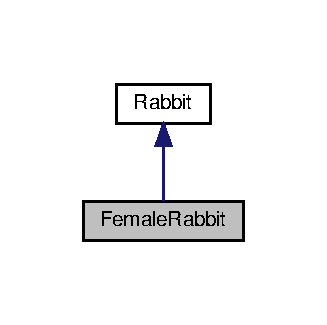
\includegraphics[width=157pt]{classFemaleRabbit__inherit__graph}
\end{center}
\end{figure}


Graphe de collaboration de Female\+Rabbit\+:
\nopagebreak
\begin{figure}[H]
\begin{center}
\leavevmode
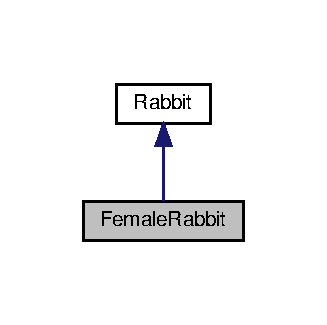
\includegraphics[width=157pt]{classFemaleRabbit__coll__graph}
\end{center}
\end{figure}
\subsection*{Fonctions membres publiques}
\begin{DoxyCompactItemize}
\item 
\hyperlink{classFemaleRabbit_a40a2809fb73bb2edf2cf4c4d9147d2d9}{Female\+Rabbit} (std\+::list$<$ \hyperlink{classRabbit}{Rabbit} $\ast$$>$ \&pop)
\begin{DoxyCompactList}\small\item\em Construit un nouvel objet \char`\"{}\+Female Rabbit\char`\"{}. \end{DoxyCompactList}\item 
\hyperlink{classFemaleRabbit_a952455c7b721ab6acb770078aa5b8d5d}{$\sim$\+Female\+Rabbit} ()
\begin{DoxyCompactList}\small\item\em Détruit l\textquotesingle{}objet \char`\"{}\+Female Rabbit\char`\"{}. \end{DoxyCompactList}\item 
virtual void \hyperlink{classFemaleRabbit_ad938ea7eca97c53e89d11392b6856ebd}{grow} ()
\begin{DoxyCompactList}\small\item\em Méthode faisant vieillir le lapin de 1 mois. \end{DoxyCompactList}\item 
virtual bool \hyperlink{classFemaleRabbit_a60250dbc3758c7d31537f13b4879fe33}{is\+Male} () const
\begin{DoxyCompactList}\small\item\em Méthode permettant de savoir si l\textquotesingle{}instance est celle d\textquotesingle{}un lapin mâle ou femelle. \end{DoxyCompactList}\end{DoxyCompactItemize}
\subsection*{Membres hérités additionnels}


\subsection{Description détaillée}
Classe représentant un lapin femelle. 

Définition à la ligne 22 du fichier Female\+Rabbit.\+hpp.



\subsection{Documentation des constructeurs et destructeur}
\mbox{\Hypertarget{classFemaleRabbit_a40a2809fb73bb2edf2cf4c4d9147d2d9}\label{classFemaleRabbit_a40a2809fb73bb2edf2cf4c4d9147d2d9}} 
\index{Female\+Rabbit@{Female\+Rabbit}!Female\+Rabbit@{Female\+Rabbit}}
\index{Female\+Rabbit@{Female\+Rabbit}!Female\+Rabbit@{Female\+Rabbit}}
\subsubsection{\texorpdfstring{Female\+Rabbit()}{FemaleRabbit()}}
{\footnotesize\ttfamily Female\+Rabbit\+::\+Female\+Rabbit (\begin{DoxyParamCaption}\item[{std\+::list$<$ \hyperlink{classRabbit}{Rabbit} $\ast$$>$ \&}]{pop }\end{DoxyParamCaption})}



Construit un nouvel objet \char`\"{}\+Female Rabbit\char`\"{}. 

Le constructeur de \hyperlink{classFemaleRabbit}{Female\+Rabbit} appelle le constructeur de \hyperlink{classRabbit}{Rabbit} afin d\textquotesingle{}initialiser les variables (telles que l\textquotesingle{}âge et les probabilités de mourir)


\begin{DoxyParams}[1]{Paramètres}
\mbox{\tt in}  & {\em pop} & liste représentant la population de lapins où la femelle créée devra enfanter \\
\hline
\end{DoxyParams}


Définition à la ligne 20 du fichier Female\+Rabbit.\+cpp.

Voici le graphe des appelants de cette fonction \+:
\nopagebreak
\begin{figure}[H]
\begin{center}
\leavevmode
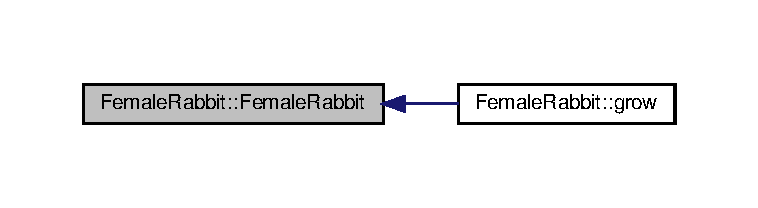
\includegraphics[width=350pt]{classFemaleRabbit_a40a2809fb73bb2edf2cf4c4d9147d2d9_icgraph}
\end{center}
\end{figure}
\mbox{\Hypertarget{classFemaleRabbit_a952455c7b721ab6acb770078aa5b8d5d}\label{classFemaleRabbit_a952455c7b721ab6acb770078aa5b8d5d}} 
\index{Female\+Rabbit@{Female\+Rabbit}!````~Female\+Rabbit@{$\sim$\+Female\+Rabbit}}
\index{````~Female\+Rabbit@{$\sim$\+Female\+Rabbit}!Female\+Rabbit@{Female\+Rabbit}}
\subsubsection{\texorpdfstring{$\sim$\+Female\+Rabbit()}{~FemaleRabbit()}}
{\footnotesize\ttfamily Female\+Rabbit\+::$\sim$\+Female\+Rabbit (\begin{DoxyParamCaption}{ }\end{DoxyParamCaption})}



Détruit l\textquotesingle{}objet \char`\"{}\+Female Rabbit\char`\"{}. 



Définition à la ligne 31 du fichier Female\+Rabbit.\+cpp.



\subsection{Documentation des fonctions membres}
\mbox{\Hypertarget{classFemaleRabbit_ad938ea7eca97c53e89d11392b6856ebd}\label{classFemaleRabbit_ad938ea7eca97c53e89d11392b6856ebd}} 
\index{Female\+Rabbit@{Female\+Rabbit}!grow@{grow}}
\index{grow@{grow}!Female\+Rabbit@{Female\+Rabbit}}
\subsubsection{\texorpdfstring{grow()}{grow()}}
{\footnotesize\ttfamily void Female\+Rabbit\+::grow (\begin{DoxyParamCaption}{ }\end{DoxyParamCaption})\hspace{0.3cm}{\ttfamily [virtual]}}



Méthode faisant vieillir le lapin de 1 mois. 

Appelle la méthode grow de \hyperlink{classRabbit}{Rabbit} afin de grandir en tant que lapin Si c\textquotesingle{}est l\textquotesingle{}anniversaire de la lapine, les mois auquels elle enfante dans l\textquotesingle{}année sont choisis Si c\textquotesingle{}est un mois où elle doit enfanter, le nombre de bébés lapins dans la portée est décidé et elle rajoute ce nombre de nouveaux lapins à la population 

Réimplémentée à partir de \hyperlink{classRabbit_a404af8877c99ddc98108d88c8e466013}{Rabbit}.



Définition à la ligne 42 du fichier Female\+Rabbit.\+cpp.

Voici le graphe d\textquotesingle{}appel pour cette fonction \+:
\nopagebreak
\begin{figure}[H]
\begin{center}
\leavevmode
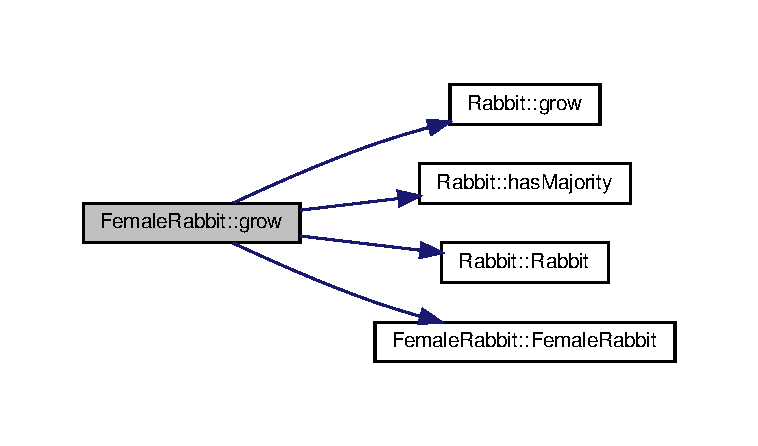
\includegraphics[width=350pt]{classFemaleRabbit_ad938ea7eca97c53e89d11392b6856ebd_cgraph}
\end{center}
\end{figure}
\mbox{\Hypertarget{classFemaleRabbit_a60250dbc3758c7d31537f13b4879fe33}\label{classFemaleRabbit_a60250dbc3758c7d31537f13b4879fe33}} 
\index{Female\+Rabbit@{Female\+Rabbit}!is\+Male@{is\+Male}}
\index{is\+Male@{is\+Male}!Female\+Rabbit@{Female\+Rabbit}}
\subsubsection{\texorpdfstring{is\+Male()}{isMale()}}
{\footnotesize\ttfamily bool Female\+Rabbit\+::is\+Male (\begin{DoxyParamCaption}{ }\end{DoxyParamCaption}) const\hspace{0.3cm}{\ttfamily [virtual]}}



Méthode permettant de savoir si l\textquotesingle{}instance est celle d\textquotesingle{}un lapin mâle ou femelle. 



Réimplémentée à partir de \hyperlink{classRabbit_a913437a589519afdb9249825bd6f03bd}{Rabbit}.



Définition à la ligne 84 du fichier Female\+Rabbit.\+cpp.



La documentation de cette classe a été générée à partir des fichiers suivants \+:\begin{DoxyCompactItemize}
\item 
\hyperlink{FemaleRabbit_8hpp}{Female\+Rabbit.\+hpp}\item 
\hyperlink{FemaleRabbit_8cpp}{Female\+Rabbit.\+cpp}\end{DoxyCompactItemize}

\hypertarget{classPopulation}{}\section{Référence de la classe Population}
\label{classPopulation}\index{Population@{Population}}


Représente une population de lapins.  




{\ttfamily \#include $<$Population.\+hpp$>$}

\subsection*{Fonctions membres publiques}
\begin{DoxyCompactItemize}
\item 
\hyperlink{classPopulation_a54eb24ca89470eebe0c27bcb03a0ceae}{Population} ()
\begin{DoxyCompactList}\small\item\em Construit un nouvel objet \char`\"{}\+Population\char`\"{}. \end{DoxyCompactList}\item 
\hyperlink{classPopulation_a8bf0924406fb56bb5177016d5ebd7911}{Population} (unsigned int number\+Of\+Male, unsigned int number\+Of\+Female)
\begin{DoxyCompactList}\small\item\em Construit un nouvel objet \char`\"{}\+Population\char`\"{}. \end{DoxyCompactList}\item 
\hyperlink{classPopulation_a4c8cedd0f038e41746fb6084639f5616}{$\sim$\+Population} ()
\begin{DoxyCompactList}\small\item\em Détruit l\textquotesingle{}objet \char`\"{}\+Population\char`\"{}. \end{DoxyCompactList}\item 
void \hyperlink{classPopulation_a4a4eef2f12f2f46c1fafef5ca4db2933}{pass\+Time} (unsigned int nb\+Of\+Months)
\begin{DoxyCompactList}\small\item\em passe le temps pour la population de lapins \end{DoxyCompactList}\item 
unsigned int \hyperlink{classPopulation_a509a07b43df688b3b3235f586e5b3c07}{get\+Month} () const
\begin{DoxyCompactList}\small\item\em getter pour le nombre de mois passés par la population \end{DoxyCompactList}\item 
size\+\_\+t \hyperlink{classPopulation_a7388e8d8308abe505b7fa95c759a03ea}{get\+Number\+Of\+Rabbit} () const
\begin{DoxyCompactList}\small\item\em getter pour le nombre de lapins de la population à l\textquotesingle{}instant t \end{DoxyCompactList}\item 
size\+\_\+t \hyperlink{classPopulation_a13d2cee6f6bf940eea261b61c5999e1f}{get\+Number\+Of\+Female\+Rabbit} () const
\begin{DoxyCompactList}\small\item\em getter pour le nombre de femelles dans la poplation à l\textquotesingle{}instant t \end{DoxyCompactList}\item 
size\+\_\+t \hyperlink{classPopulation_a74dc9a5e829548a16d7910d7c17bb751}{get\+Number\+Of\+Male\+Rabbit} () const
\begin{DoxyCompactList}\small\item\em getter pour le nombre de mâles dans la poplation à l\textquotesingle{}instant t \end{DoxyCompactList}\item 
size\+\_\+t \hyperlink{classPopulation_a8cf700f7fa2dfd54035322c05bfc9914}{get\+Death} () const
\begin{DoxyCompactList}\small\item\em getter pour le nombre de morts depuis le début de la population \end{DoxyCompactList}\item 
size\+\_\+t \hyperlink{classPopulation_a703218d79e0d156a10c19e70d7433fa9}{get\+Birth} () const
\begin{DoxyCompactList}\small\item\em getter pour le nombre de naissances depuis le début de la population \end{DoxyCompactList}\item 
double \hyperlink{classPopulation_aa5a0becf703f219c9e1a4270d54c397e}{get\+Mean\+Death\+Age} () const
\begin{DoxyCompactList}\small\item\em getter pour la moyenne d\textquotesingle{}age auquel les lapins meurent \end{DoxyCompactList}\item 
void \hyperlink{classPopulation_a4c7cc56a0bce95aa909bc75df7043f1a}{export\+To\+C\+SV} (std\+::string const \&filename)
\begin{DoxyCompactList}\small\item\em ecrit dans un fichier les statistiques de la population à l\textquotesingle{}instant t \end{DoxyCompactList}\end{DoxyCompactItemize}


\subsection{Description détaillée}
Représente une population de lapins. 

Définition à la ligne 24 du fichier Population.\+hpp.



\subsection{Documentation des constructeurs et destructeur}
\mbox{\Hypertarget{classPopulation_a54eb24ca89470eebe0c27bcb03a0ceae}\label{classPopulation_a54eb24ca89470eebe0c27bcb03a0ceae}} 
\index{Population@{Population}!Population@{Population}}
\index{Population@{Population}!Population@{Population}}
\subsubsection{\texorpdfstring{Population()}{Population()}\hspace{0.1cm}{\footnotesize\ttfamily [1/2]}}
{\footnotesize\ttfamily Population\+::\+Population (\begin{DoxyParamCaption}{ }\end{DoxyParamCaption})}



Construit un nouvel objet \char`\"{}\+Population\char`\"{}. 

Initialise la population avec 1 lapin mâle et 1 lapin femelle 

Définition à la ligne 18 du fichier Population.\+cpp.

\mbox{\Hypertarget{classPopulation_a8bf0924406fb56bb5177016d5ebd7911}\label{classPopulation_a8bf0924406fb56bb5177016d5ebd7911}} 
\index{Population@{Population}!Population@{Population}}
\index{Population@{Population}!Population@{Population}}
\subsubsection{\texorpdfstring{Population()}{Population()}\hspace{0.1cm}{\footnotesize\ttfamily [2/2]}}
{\footnotesize\ttfamily Population\+::\+Population (\begin{DoxyParamCaption}\item[{unsigned int}]{number\+Of\+Male,  }\item[{unsigned int}]{number\+Of\+Female }\end{DoxyParamCaption})}



Construit un nouvel objet \char`\"{}\+Population\char`\"{}. 

Initialise la population avec un nombre spécifié de mâles et de femelles


\begin{DoxyParams}[1]{Paramètres}
\mbox{\tt in}  & {\em number\+Of\+Male} & nombre de mâles à la date 0 dans la population \\
\hline
\mbox{\tt in}  & {\em number\+Of\+Female} & nombre de femelles à la date 0 dans la population \\
\hline
\end{DoxyParams}


Définition à la ligne 36 du fichier Population.\+cpp.

\mbox{\Hypertarget{classPopulation_a4c8cedd0f038e41746fb6084639f5616}\label{classPopulation_a4c8cedd0f038e41746fb6084639f5616}} 
\index{Population@{Population}!````~Population@{$\sim$\+Population}}
\index{````~Population@{$\sim$\+Population}!Population@{Population}}
\subsubsection{\texorpdfstring{$\sim$\+Population()}{~Population()}}
{\footnotesize\ttfamily Population\+::$\sim$\+Population (\begin{DoxyParamCaption}{ }\end{DoxyParamCaption})}



Détruit l\textquotesingle{}objet \char`\"{}\+Population\char`\"{}. 

Désalloue la mémoire allouée par les lapins de la population 

Définition à la ligne 54 du fichier Population.\+cpp.



\subsection{Documentation des fonctions membres}
\mbox{\Hypertarget{classPopulation_a4c7cc56a0bce95aa909bc75df7043f1a}\label{classPopulation_a4c7cc56a0bce95aa909bc75df7043f1a}} 
\index{Population@{Population}!export\+To\+C\+SV@{export\+To\+C\+SV}}
\index{export\+To\+C\+SV@{export\+To\+C\+SV}!Population@{Population}}
\subsubsection{\texorpdfstring{export\+To\+C\+S\+V()}{exportToCSV()}}
{\footnotesize\ttfamily void Population\+::export\+To\+C\+SV (\begin{DoxyParamCaption}\item[{std\+::string const \&}]{filename }\end{DoxyParamCaption})}



ecrit dans un fichier les statistiques de la population à l\textquotesingle{}instant t 


\begin{DoxyParams}[1]{Paramètres}
\mbox{\tt in}  & {\em filename} & nom du fichier dans lequel on ajoute une ligne de statistiques \\
\hline
\end{DoxyParams}


Définition à la ligne 187 du fichier Population.\+cpp.

Voici le graphe d\textquotesingle{}appel pour cette fonction \+:
\nopagebreak
\begin{figure}[H]
\begin{center}
\leavevmode
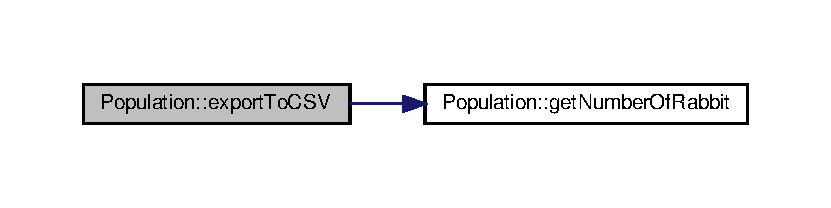
\includegraphics[width=350pt]{classPopulation_a4c7cc56a0bce95aa909bc75df7043f1a_cgraph}
\end{center}
\end{figure}
\mbox{\Hypertarget{classPopulation_a703218d79e0d156a10c19e70d7433fa9}\label{classPopulation_a703218d79e0d156a10c19e70d7433fa9}} 
\index{Population@{Population}!get\+Birth@{get\+Birth}}
\index{get\+Birth@{get\+Birth}!Population@{Population}}
\subsubsection{\texorpdfstring{get\+Birth()}{getBirth()}}
{\footnotesize\ttfamily size\+\_\+t Population\+::get\+Birth (\begin{DoxyParamCaption}{ }\end{DoxyParamCaption}) const}



getter pour le nombre de naissances depuis le début de la population 

\begin{DoxyReturn}{Renvoie}
size\+\_\+t nombre de naissances 
\end{DoxyReturn}


Définition à la ligne 167 du fichier Population.\+cpp.

Voici le graphe des appelants de cette fonction \+:
\nopagebreak
\begin{figure}[H]
\begin{center}
\leavevmode
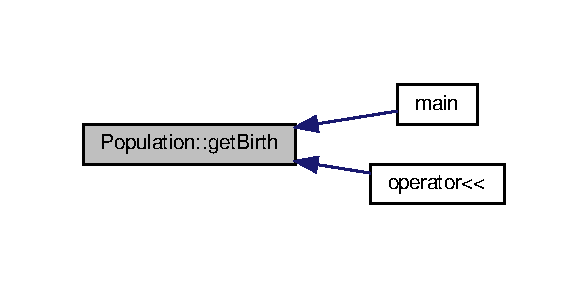
\includegraphics[width=282pt]{classPopulation_a703218d79e0d156a10c19e70d7433fa9_icgraph}
\end{center}
\end{figure}
\mbox{\Hypertarget{classPopulation_a8cf700f7fa2dfd54035322c05bfc9914}\label{classPopulation_a8cf700f7fa2dfd54035322c05bfc9914}} 
\index{Population@{Population}!get\+Death@{get\+Death}}
\index{get\+Death@{get\+Death}!Population@{Population}}
\subsubsection{\texorpdfstring{get\+Death()}{getDeath()}}
{\footnotesize\ttfamily size\+\_\+t Population\+::get\+Death (\begin{DoxyParamCaption}{ }\end{DoxyParamCaption}) const}



getter pour le nombre de morts depuis le début de la population 

\begin{DoxyReturn}{Renvoie}
size\+\_\+t nombre de morts 
\end{DoxyReturn}


Définition à la ligne 157 du fichier Population.\+cpp.

Voici le graphe des appelants de cette fonction \+:
\nopagebreak
\begin{figure}[H]
\begin{center}
\leavevmode
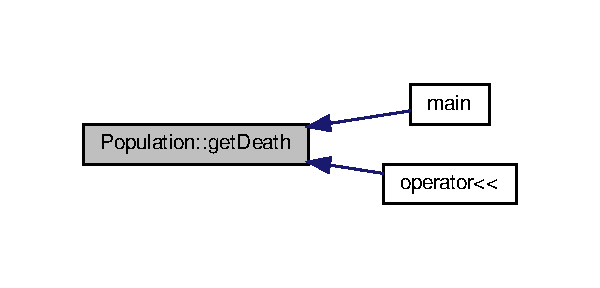
\includegraphics[width=288pt]{classPopulation_a8cf700f7fa2dfd54035322c05bfc9914_icgraph}
\end{center}
\end{figure}
\mbox{\Hypertarget{classPopulation_aa5a0becf703f219c9e1a4270d54c397e}\label{classPopulation_aa5a0becf703f219c9e1a4270d54c397e}} 
\index{Population@{Population}!get\+Mean\+Death\+Age@{get\+Mean\+Death\+Age}}
\index{get\+Mean\+Death\+Age@{get\+Mean\+Death\+Age}!Population@{Population}}
\subsubsection{\texorpdfstring{get\+Mean\+Death\+Age()}{getMeanDeathAge()}}
{\footnotesize\ttfamily double Population\+::get\+Mean\+Death\+Age (\begin{DoxyParamCaption}{ }\end{DoxyParamCaption}) const}



getter pour la moyenne d\textquotesingle{}age auquel les lapins meurent 

\begin{DoxyReturn}{Renvoie}
double moyenne d\textquotesingle{}age de mort 
\end{DoxyReturn}


Définition à la ligne 177 du fichier Population.\+cpp.

Voici le graphe des appelants de cette fonction \+:
\nopagebreak
\begin{figure}[H]
\begin{center}
\leavevmode
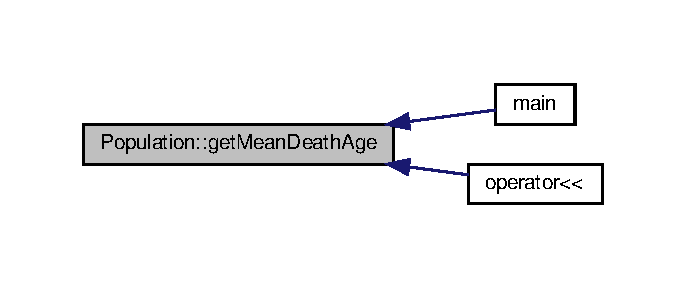
\includegraphics[width=329pt]{classPopulation_aa5a0becf703f219c9e1a4270d54c397e_icgraph}
\end{center}
\end{figure}
\mbox{\Hypertarget{classPopulation_a509a07b43df688b3b3235f586e5b3c07}\label{classPopulation_a509a07b43df688b3b3235f586e5b3c07}} 
\index{Population@{Population}!get\+Month@{get\+Month}}
\index{get\+Month@{get\+Month}!Population@{Population}}
\subsubsection{\texorpdfstring{get\+Month()}{getMonth()}}
{\footnotesize\ttfamily unsigned int Population\+::get\+Month (\begin{DoxyParamCaption}{ }\end{DoxyParamCaption}) const}



getter pour le nombre de mois passés par la population 

\begin{DoxyReturn}{Renvoie}
unsigned int nombre de mois passés par la population 
\end{DoxyReturn}


Définition à la ligne 105 du fichier Population.\+cpp.

\mbox{\Hypertarget{classPopulation_a13d2cee6f6bf940eea261b61c5999e1f}\label{classPopulation_a13d2cee6f6bf940eea261b61c5999e1f}} 
\index{Population@{Population}!get\+Number\+Of\+Female\+Rabbit@{get\+Number\+Of\+Female\+Rabbit}}
\index{get\+Number\+Of\+Female\+Rabbit@{get\+Number\+Of\+Female\+Rabbit}!Population@{Population}}
\subsubsection{\texorpdfstring{get\+Number\+Of\+Female\+Rabbit()}{getNumberOfFemaleRabbit()}}
{\footnotesize\ttfamily size\+\_\+t Population\+::get\+Number\+Of\+Female\+Rabbit (\begin{DoxyParamCaption}{ }\end{DoxyParamCaption}) const}



getter pour le nombre de femelles dans la poplation à l\textquotesingle{}instant t 

\begin{DoxyReturn}{Renvoie}
size\+\_\+t nombre de lapins femelles dans la population 
\end{DoxyReturn}


Définition à la ligne 125 du fichier Population.\+cpp.

Voici le graphe des appelants de cette fonction \+:
\nopagebreak
\begin{figure}[H]
\begin{center}
\leavevmode
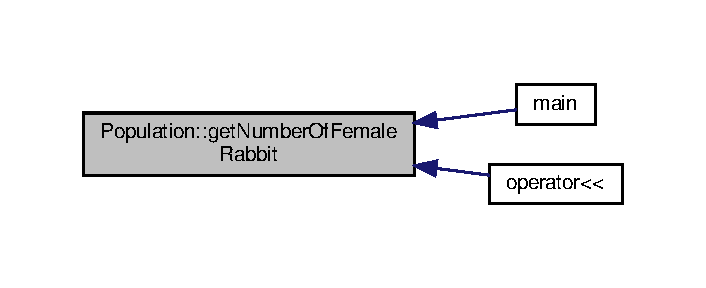
\includegraphics[width=339pt]{classPopulation_a13d2cee6f6bf940eea261b61c5999e1f_icgraph}
\end{center}
\end{figure}
\mbox{\Hypertarget{classPopulation_a74dc9a5e829548a16d7910d7c17bb751}\label{classPopulation_a74dc9a5e829548a16d7910d7c17bb751}} 
\index{Population@{Population}!get\+Number\+Of\+Male\+Rabbit@{get\+Number\+Of\+Male\+Rabbit}}
\index{get\+Number\+Of\+Male\+Rabbit@{get\+Number\+Of\+Male\+Rabbit}!Population@{Population}}
\subsubsection{\texorpdfstring{get\+Number\+Of\+Male\+Rabbit()}{getNumberOfMaleRabbit()}}
{\footnotesize\ttfamily size\+\_\+t Population\+::get\+Number\+Of\+Male\+Rabbit (\begin{DoxyParamCaption}{ }\end{DoxyParamCaption}) const}



getter pour le nombre de mâles dans la poplation à l\textquotesingle{}instant t 

\begin{DoxyReturn}{Renvoie}
size\+\_\+t nombre de lapins mâles dans la population 
\end{DoxyReturn}


Définition à la ligne 141 du fichier Population.\+cpp.

Voici le graphe des appelants de cette fonction \+:
\nopagebreak
\begin{figure}[H]
\begin{center}
\leavevmode
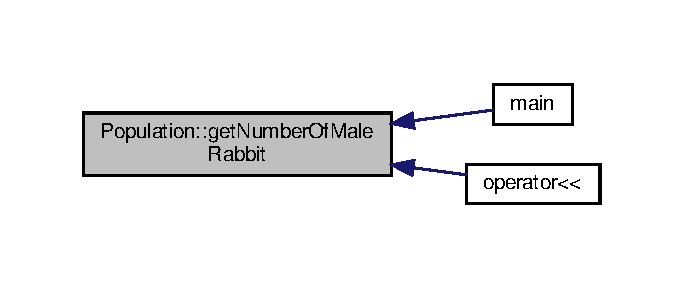
\includegraphics[width=328pt]{classPopulation_a74dc9a5e829548a16d7910d7c17bb751_icgraph}
\end{center}
\end{figure}
\mbox{\Hypertarget{classPopulation_a7388e8d8308abe505b7fa95c759a03ea}\label{classPopulation_a7388e8d8308abe505b7fa95c759a03ea}} 
\index{Population@{Population}!get\+Number\+Of\+Rabbit@{get\+Number\+Of\+Rabbit}}
\index{get\+Number\+Of\+Rabbit@{get\+Number\+Of\+Rabbit}!Population@{Population}}
\subsubsection{\texorpdfstring{get\+Number\+Of\+Rabbit()}{getNumberOfRabbit()}}
{\footnotesize\ttfamily size\+\_\+t Population\+::get\+Number\+Of\+Rabbit (\begin{DoxyParamCaption}{ }\end{DoxyParamCaption}) const}



getter pour le nombre de lapins de la population à l\textquotesingle{}instant t 

\begin{DoxyReturn}{Renvoie}
size\+\_\+t nombre de lapins (vivants) dans la population 
\end{DoxyReturn}


Définition à la ligne 115 du fichier Population.\+cpp.

Voici le graphe des appelants de cette fonction \+:
\nopagebreak
\begin{figure}[H]
\begin{center}
\leavevmode
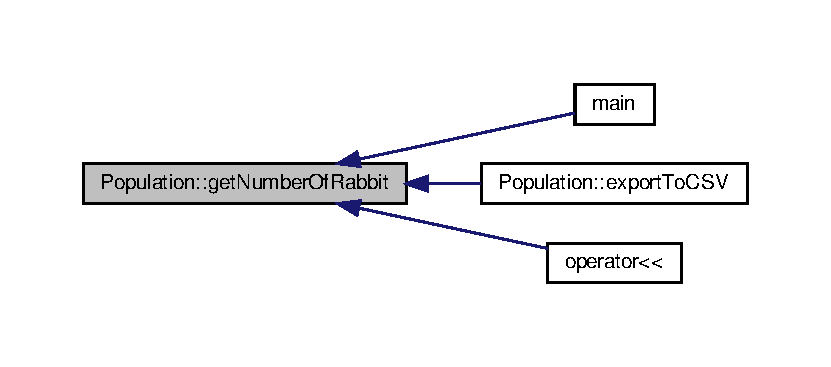
\includegraphics[width=350pt]{classPopulation_a7388e8d8308abe505b7fa95c759a03ea_icgraph}
\end{center}
\end{figure}
\mbox{\Hypertarget{classPopulation_a4a4eef2f12f2f46c1fafef5ca4db2933}\label{classPopulation_a4a4eef2f12f2f46c1fafef5ca4db2933}} 
\index{Population@{Population}!pass\+Time@{pass\+Time}}
\index{pass\+Time@{pass\+Time}!Population@{Population}}
\subsubsection{\texorpdfstring{pass\+Time()}{passTime()}}
{\footnotesize\ttfamily void Population\+::pass\+Time (\begin{DoxyParamCaption}\item[{unsigned int}]{nb\+Of\+Months }\end{DoxyParamCaption})}



passe le temps pour la population de lapins 

Passe un nombre de mois spécifié pour tous les lapins de la population La méthode les fait grandir avec la fonction grow, et si des lapins meurent, les supprime de la liste


\begin{DoxyParams}[1]{Paramètres}
\mbox{\tt in}  & {\em nb\+Of\+Months} & nombre de mois que l\textquotesingle{}on veut passer \\
\hline
\end{DoxyParams}


Définition à la ligne 67 du fichier Population.\+cpp.

Voici le graphe des appelants de cette fonction \+:
\nopagebreak
\begin{figure}[H]
\begin{center}
\leavevmode
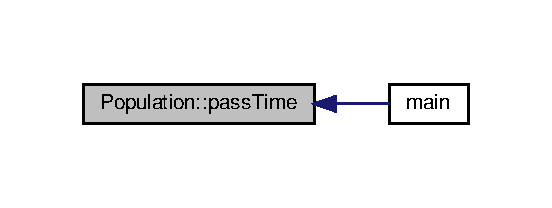
\includegraphics[width=265pt]{classPopulation_a4a4eef2f12f2f46c1fafef5ca4db2933_icgraph}
\end{center}
\end{figure}


La documentation de cette classe a été générée à partir des fichiers suivants \+:\begin{DoxyCompactItemize}
\item 
\hyperlink{Population_8hpp}{Population.\+hpp}\item 
\hyperlink{Population_8cpp}{Population.\+cpp}\end{DoxyCompactItemize}

\hypertarget{classRabbit}{}\section{Référence de la classe Rabbit}
\label{classRabbit}\index{Rabbit@{Rabbit}}


Classe représentant un lapin (mâle ou femelle)  




{\ttfamily \#include $<$Rabbit.\+hpp$>$}



Graphe d\textquotesingle{}héritage de Rabbit\+:
\nopagebreak
\begin{figure}[H]
\begin{center}
\leavevmode
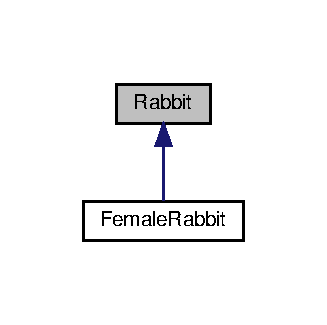
\includegraphics[width=157pt]{classRabbit__inherit__graph}
\end{center}
\end{figure}
\subsection*{Fonctions membres publiques}
\begin{DoxyCompactItemize}
\item 
\hyperlink{classRabbit_ae2093988d2ba8f561213a9767e8a31dd}{Rabbit} ()
\begin{DoxyCompactList}\small\item\em Construit un nouvel objet \char`\"{}\+Rabbit\char`\"{}. \end{DoxyCompactList}\item 
virtual \hyperlink{classRabbit_ac57586ffc31fffa6392638afbbd32774}{$\sim$\+Rabbit} ()
\begin{DoxyCompactList}\small\item\em Détruit l\textquotesingle{}objet \char`\"{}\+Rabbit\char`\"{}. \end{DoxyCompactList}\item 
virtual void \hyperlink{classRabbit_a404af8877c99ddc98108d88c8e466013}{grow} ()
\begin{DoxyCompactList}\small\item\em Méthode qui fait veillir l\textquotesingle{}instance d\textquotesingle{}un lapin de 1 mois. \end{DoxyCompactList}\item 
bool \hyperlink{classRabbit_a8087ee3ab0acaa6108e6982933b0f79a}{has\+Majority} () const
\begin{DoxyCompactList}\small\item\em Méthode pour savoir si le lapin est jeune ou adulte. \end{DoxyCompactList}\item 
bool \hyperlink{classRabbit_a82cf75bd520aaa775fadbf103fc12499}{has\+To\+Die} () const
\begin{DoxyCompactList}\small\item\em Méthode pour savoir si le lapin doit mourir ce mois. \end{DoxyCompactList}\item 
unsigned int \hyperlink{classRabbit_ab34450717cf7b3f9eb22747527c34922}{get\+Age} () const
\begin{DoxyCompactList}\small\item\em Getter pour l\textquotesingle{}age. \end{DoxyCompactList}\item 
virtual bool \hyperlink{classRabbit_a913437a589519afdb9249825bd6f03bd}{is\+Male} () const
\begin{DoxyCompactList}\small\item\em Méthode permettant de savoir si l\textquotesingle{}instance est celle d\textquotesingle{}un lapin mâle ou femelle. \end{DoxyCompactList}\end{DoxyCompactItemize}
\subsection*{Attributs publics statiques}
\begin{DoxyCompactItemize}
\item 
static constexpr double \hyperlink{classRabbit_ac6dc736f2b0395fa8692461a457a5297}{survival\+\_\+proba\+\_\+young} = 0.\+2
\begin{DoxyCompactList}\small\item\em probabilité de survivre à la jeunesse (les 5 à 8 premiers mois) \end{DoxyCompactList}\item 
static constexpr double \hyperlink{classRabbit_a8b8affe7fcdc56e08da384d8d82ec556}{survival\+\_\+proba\+\_\+adult} = 0.\+5
\begin{DoxyCompactList}\small\item\em probabilité de survivre pour un lapin adulte (11 ans moins les mois de jeunesse) \end{DoxyCompactList}\end{DoxyCompactItemize}
\subsection*{Attributs protégés}
\begin{DoxyCompactItemize}
\item 
unsigned int \hyperlink{classRabbit_a396c4c8693ea4f827f12afd6d1320ec0}{\+\_\+age}
\begin{DoxyCompactList}\small\item\em L\textquotesingle{}age du lapin en mois. \end{DoxyCompactList}\item 
unsigned int \hyperlink{classRabbit_a7cf441478e82d384166605c69f99f39e}{\+\_\+majority}
\begin{DoxyCompactList}\small\item\em Nombre de mois avant que le lapin n\textquotesingle{}atteigne la majorité et passe à l\textquotesingle{}age adulte et puisse enfanter (si c\textquotesingle{}est une femelle) \end{DoxyCompactList}\item 
double \hyperlink{classRabbit_a622452eedf7ef0addf1e2ce3d8ef34dc}{\+\_\+proba\+\_\+to\+\_\+die\+\_\+young}
\begin{DoxyCompactList}\small\item\em Probabilité de mourir (par mois) avant de devenir adulte, calculée avec la probabilité de survivre et le nombre de mois de jeunesse. \end{DoxyCompactList}\item 
double \hyperlink{classRabbit_a600d8595c407b95965497f7308d72ab1}{\+\_\+proba\+\_\+to\+\_\+die\+\_\+adult}
\begin{DoxyCompactList}\small\item\em Probabilité de mourir (par mois) en étant adulte, calculée avec la probabilité de survivre et le nombre de mois de jeunesse. \end{DoxyCompactList}\end{DoxyCompactItemize}


\subsection{Description détaillée}
Classe représentant un lapin (mâle ou femelle) 

Si l\textquotesingle{}objet est créé en tant que \hyperlink{classRabbit}{Rabbit}, c\textquotesingle{}est qu\textquotesingle{}il représente un lapin mâle, sinon la classe utilisée sera \hyperlink{classFemaleRabbit}{Female\+Rabbit}. Cependant la classe \hyperlink{classRabbit}{Rabbit} synthétise les deux genres. Il n\textquotesingle{}y a juste pas de classe Male\+Rabbit puisque celle-\/ci n\textquotesingle{}implémenterait rien de plus que la classe \hyperlink{classRabbit}{Rabbit}. 

Définition à la ligne 23 du fichier Rabbit.\+hpp.



\subsection{Documentation des constructeurs et destructeur}
\mbox{\Hypertarget{classRabbit_ae2093988d2ba8f561213a9767e8a31dd}\label{classRabbit_ae2093988d2ba8f561213a9767e8a31dd}} 
\index{Rabbit@{Rabbit}!Rabbit@{Rabbit}}
\index{Rabbit@{Rabbit}!Rabbit@{Rabbit}}
\subsubsection{\texorpdfstring{Rabbit()}{Rabbit()}}
{\footnotesize\ttfamily Rabbit\+::\+Rabbit (\begin{DoxyParamCaption}{ }\end{DoxyParamCaption})}



Construit un nouvel objet \char`\"{}\+Rabbit\char`\"{}. 

Définit l\textquotesingle{}age de la majorité, la probabilité de mourir jeune et la probabilité de mourir en étant adulte 

Définition à la ligne 18 du fichier Rabbit.\+cpp.

Voici le graphe des appelants de cette fonction \+:
\nopagebreak
\begin{figure}[H]
\begin{center}
\leavevmode
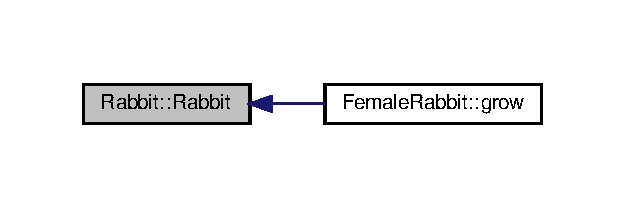
\includegraphics[width=300pt]{classRabbit_ae2093988d2ba8f561213a9767e8a31dd_icgraph}
\end{center}
\end{figure}
\mbox{\Hypertarget{classRabbit_ac57586ffc31fffa6392638afbbd32774}\label{classRabbit_ac57586ffc31fffa6392638afbbd32774}} 
\index{Rabbit@{Rabbit}!````~Rabbit@{$\sim$\+Rabbit}}
\index{````~Rabbit@{$\sim$\+Rabbit}!Rabbit@{Rabbit}}
\subsubsection{\texorpdfstring{$\sim$\+Rabbit()}{~Rabbit()}}
{\footnotesize\ttfamily Rabbit\+::$\sim$\+Rabbit (\begin{DoxyParamCaption}{ }\end{DoxyParamCaption})\hspace{0.3cm}{\ttfamily [virtual]}}



Détruit l\textquotesingle{}objet \char`\"{}\+Rabbit\char`\"{}. 



Définition à la ligne 29 du fichier Rabbit.\+cpp.



\subsection{Documentation des fonctions membres}
\mbox{\Hypertarget{classRabbit_ab34450717cf7b3f9eb22747527c34922}\label{classRabbit_ab34450717cf7b3f9eb22747527c34922}} 
\index{Rabbit@{Rabbit}!get\+Age@{get\+Age}}
\index{get\+Age@{get\+Age}!Rabbit@{Rabbit}}
\subsubsection{\texorpdfstring{get\+Age()}{getAge()}}
{\footnotesize\ttfamily unsigned int Rabbit\+::get\+Age (\begin{DoxyParamCaption}{ }\end{DoxyParamCaption}) const}



Getter pour l\textquotesingle{}age. 

\begin{DoxyReturn}{Renvoie}
unsigned int l\textquotesingle{}age du lapin 
\end{DoxyReturn}


Définition à la ligne 68 du fichier Rabbit.\+cpp.

\mbox{\Hypertarget{classRabbit_a404af8877c99ddc98108d88c8e466013}\label{classRabbit_a404af8877c99ddc98108d88c8e466013}} 
\index{Rabbit@{Rabbit}!grow@{grow}}
\index{grow@{grow}!Rabbit@{Rabbit}}
\subsubsection{\texorpdfstring{grow()}{grow()}}
{\footnotesize\ttfamily void Rabbit\+::grow (\begin{DoxyParamCaption}{ }\end{DoxyParamCaption})\hspace{0.3cm}{\ttfamily [virtual]}}



Méthode qui fait veillir l\textquotesingle{}instance d\textquotesingle{}un lapin de 1 mois. 



Réimplémentée dans \hyperlink{classFemaleRabbit_ad938ea7eca97c53e89d11392b6856ebd}{Female\+Rabbit}.



Définition à la ligne 36 du fichier Rabbit.\+cpp.

Voici le graphe des appelants de cette fonction \+:
\nopagebreak
\begin{figure}[H]
\begin{center}
\leavevmode
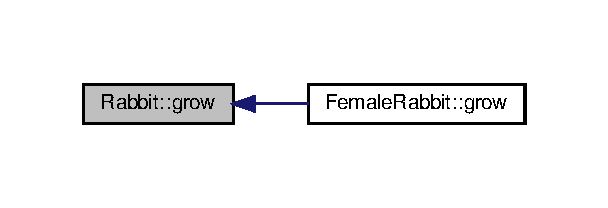
\includegraphics[width=292pt]{classRabbit_a404af8877c99ddc98108d88c8e466013_icgraph}
\end{center}
\end{figure}
\mbox{\Hypertarget{classRabbit_a8087ee3ab0acaa6108e6982933b0f79a}\label{classRabbit_a8087ee3ab0acaa6108e6982933b0f79a}} 
\index{Rabbit@{Rabbit}!has\+Majority@{has\+Majority}}
\index{has\+Majority@{has\+Majority}!Rabbit@{Rabbit}}
\subsubsection{\texorpdfstring{has\+Majority()}{hasMajority()}}
{\footnotesize\ttfamily bool Rabbit\+::has\+Majority (\begin{DoxyParamCaption}{ }\end{DoxyParamCaption}) const}



Méthode pour savoir si le lapin est jeune ou adulte. 

\begin{DoxyReturn}{Renvoie}
true si le lapin est adulte 

false si le lapin est jeune 
\end{DoxyReturn}


Définition à la ligne 47 du fichier Rabbit.\+cpp.

Voici le graphe des appelants de cette fonction \+:
\nopagebreak
\begin{figure}[H]
\begin{center}
\leavevmode
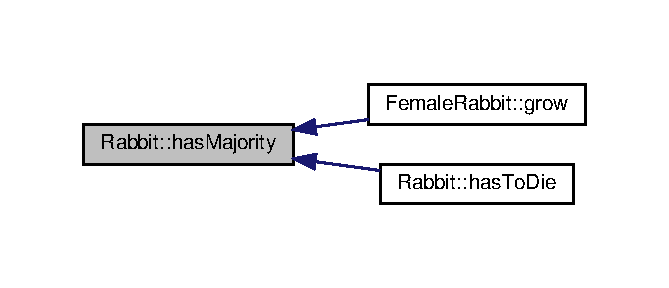
\includegraphics[width=321pt]{classRabbit_a8087ee3ab0acaa6108e6982933b0f79a_icgraph}
\end{center}
\end{figure}
\mbox{\Hypertarget{classRabbit_a82cf75bd520aaa775fadbf103fc12499}\label{classRabbit_a82cf75bd520aaa775fadbf103fc12499}} 
\index{Rabbit@{Rabbit}!has\+To\+Die@{has\+To\+Die}}
\index{has\+To\+Die@{has\+To\+Die}!Rabbit@{Rabbit}}
\subsubsection{\texorpdfstring{has\+To\+Die()}{hasToDie()}}
{\footnotesize\ttfamily bool Rabbit\+::has\+To\+Die (\begin{DoxyParamCaption}{ }\end{DoxyParamCaption}) const}



Méthode pour savoir si le lapin doit mourir ce mois. 

\begin{DoxyReturn}{Renvoie}
true si il doit mourir 

false si il survit 
\end{DoxyReturn}


Définition à la ligne 58 du fichier Rabbit.\+cpp.

Voici le graphe d\textquotesingle{}appel pour cette fonction \+:
\nopagebreak
\begin{figure}[H]
\begin{center}
\leavevmode
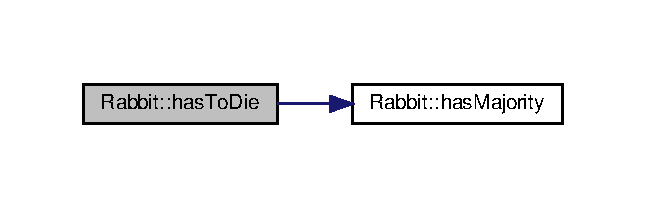
\includegraphics[width=310pt]{classRabbit_a82cf75bd520aaa775fadbf103fc12499_cgraph}
\end{center}
\end{figure}
\mbox{\Hypertarget{classRabbit_a913437a589519afdb9249825bd6f03bd}\label{classRabbit_a913437a589519afdb9249825bd6f03bd}} 
\index{Rabbit@{Rabbit}!is\+Male@{is\+Male}}
\index{is\+Male@{is\+Male}!Rabbit@{Rabbit}}
\subsubsection{\texorpdfstring{is\+Male()}{isMale()}}
{\footnotesize\ttfamily bool Rabbit\+::is\+Male (\begin{DoxyParamCaption}{ }\end{DoxyParamCaption}) const\hspace{0.3cm}{\ttfamily [virtual]}}



Méthode permettant de savoir si l\textquotesingle{}instance est celle d\textquotesingle{}un lapin mâle ou femelle. 



Réimplémentée dans \hyperlink{classFemaleRabbit_a60250dbc3758c7d31537f13b4879fe33}{Female\+Rabbit}.



Définition à la ligne 76 du fichier Rabbit.\+cpp.



\subsection{Documentation des champs}
\mbox{\Hypertarget{classRabbit_a396c4c8693ea4f827f12afd6d1320ec0}\label{classRabbit_a396c4c8693ea4f827f12afd6d1320ec0}} 
\index{Rabbit@{Rabbit}!\+\_\+age@{\+\_\+age}}
\index{\+\_\+age@{\+\_\+age}!Rabbit@{Rabbit}}
\subsubsection{\texorpdfstring{\+\_\+age}{\_age}}
{\footnotesize\ttfamily unsigned int Rabbit\+::\+\_\+age\hspace{0.3cm}{\ttfamily [protected]}}



L\textquotesingle{}age du lapin en mois. 



Définition à la ligne 39 du fichier Rabbit.\+hpp.

\mbox{\Hypertarget{classRabbit_a7cf441478e82d384166605c69f99f39e}\label{classRabbit_a7cf441478e82d384166605c69f99f39e}} 
\index{Rabbit@{Rabbit}!\+\_\+majority@{\+\_\+majority}}
\index{\+\_\+majority@{\+\_\+majority}!Rabbit@{Rabbit}}
\subsubsection{\texorpdfstring{\+\_\+majority}{\_majority}}
{\footnotesize\ttfamily unsigned int Rabbit\+::\+\_\+majority\hspace{0.3cm}{\ttfamily [protected]}}



Nombre de mois avant que le lapin n\textquotesingle{}atteigne la majorité et passe à l\textquotesingle{}age adulte et puisse enfanter (si c\textquotesingle{}est une femelle) 



Définition à la ligne 40 du fichier Rabbit.\+hpp.

\mbox{\Hypertarget{classRabbit_a600d8595c407b95965497f7308d72ab1}\label{classRabbit_a600d8595c407b95965497f7308d72ab1}} 
\index{Rabbit@{Rabbit}!\+\_\+proba\+\_\+to\+\_\+die\+\_\+adult@{\+\_\+proba\+\_\+to\+\_\+die\+\_\+adult}}
\index{\+\_\+proba\+\_\+to\+\_\+die\+\_\+adult@{\+\_\+proba\+\_\+to\+\_\+die\+\_\+adult}!Rabbit@{Rabbit}}
\subsubsection{\texorpdfstring{\+\_\+proba\+\_\+to\+\_\+die\+\_\+adult}{\_proba\_to\_die\_adult}}
{\footnotesize\ttfamily double Rabbit\+::\+\_\+proba\+\_\+to\+\_\+die\+\_\+adult\hspace{0.3cm}{\ttfamily [protected]}}



Probabilité de mourir (par mois) en étant adulte, calculée avec la probabilité de survivre et le nombre de mois de jeunesse. 



Définition à la ligne 42 du fichier Rabbit.\+hpp.

\mbox{\Hypertarget{classRabbit_a622452eedf7ef0addf1e2ce3d8ef34dc}\label{classRabbit_a622452eedf7ef0addf1e2ce3d8ef34dc}} 
\index{Rabbit@{Rabbit}!\+\_\+proba\+\_\+to\+\_\+die\+\_\+young@{\+\_\+proba\+\_\+to\+\_\+die\+\_\+young}}
\index{\+\_\+proba\+\_\+to\+\_\+die\+\_\+young@{\+\_\+proba\+\_\+to\+\_\+die\+\_\+young}!Rabbit@{Rabbit}}
\subsubsection{\texorpdfstring{\+\_\+proba\+\_\+to\+\_\+die\+\_\+young}{\_proba\_to\_die\_young}}
{\footnotesize\ttfamily double Rabbit\+::\+\_\+proba\+\_\+to\+\_\+die\+\_\+young\hspace{0.3cm}{\ttfamily [protected]}}



Probabilité de mourir (par mois) avant de devenir adulte, calculée avec la probabilité de survivre et le nombre de mois de jeunesse. 



Définition à la ligne 41 du fichier Rabbit.\+hpp.

\mbox{\Hypertarget{classRabbit_a8b8affe7fcdc56e08da384d8d82ec556}\label{classRabbit_a8b8affe7fcdc56e08da384d8d82ec556}} 
\index{Rabbit@{Rabbit}!survival\+\_\+proba\+\_\+adult@{survival\+\_\+proba\+\_\+adult}}
\index{survival\+\_\+proba\+\_\+adult@{survival\+\_\+proba\+\_\+adult}!Rabbit@{Rabbit}}
\subsubsection{\texorpdfstring{survival\+\_\+proba\+\_\+adult}{survival\_proba\_adult}}
{\footnotesize\ttfamily constexpr double Rabbit\+::survival\+\_\+proba\+\_\+adult = 0.\+5\hspace{0.3cm}{\ttfamily [static]}}



probabilité de survivre pour un lapin adulte (11 ans moins les mois de jeunesse) 



Définition à la ligne 36 du fichier Rabbit.\+hpp.

\mbox{\Hypertarget{classRabbit_ac6dc736f2b0395fa8692461a457a5297}\label{classRabbit_ac6dc736f2b0395fa8692461a457a5297}} 
\index{Rabbit@{Rabbit}!survival\+\_\+proba\+\_\+young@{survival\+\_\+proba\+\_\+young}}
\index{survival\+\_\+proba\+\_\+young@{survival\+\_\+proba\+\_\+young}!Rabbit@{Rabbit}}
\subsubsection{\texorpdfstring{survival\+\_\+proba\+\_\+young}{survival\_proba\_young}}
{\footnotesize\ttfamily constexpr double Rabbit\+::survival\+\_\+proba\+\_\+young = 0.\+2\hspace{0.3cm}{\ttfamily [static]}}



probabilité de survivre à la jeunesse (les 5 à 8 premiers mois) 



Définition à la ligne 35 du fichier Rabbit.\+hpp.



La documentation de cette classe a été générée à partir des fichiers suivants \+:\begin{DoxyCompactItemize}
\item 
\hyperlink{Rabbit_8hpp}{Rabbit.\+hpp}\item 
\hyperlink{Rabbit_8cpp}{Rabbit.\+cpp}\end{DoxyCompactItemize}

\chapter{Documentation des fichiers}
\hypertarget{FemaleRabbit_8cpp}{}\section{Référence du fichier Female\+Rabbit.\+cpp}
\label{FemaleRabbit_8cpp}\index{Female\+Rabbit.\+cpp@{Female\+Rabbit.\+cpp}}


Fichier d\textquotesingle{}implémentation de la classe \hyperlink{classFemaleRabbit}{Female\+Rabbit}.  


{\ttfamily \#include \char`\"{}Female\+Rabbit.\+hpp\char`\"{}}\newline
Graphe des dépendances par inclusion de Female\+Rabbit.\+cpp\+:
\nopagebreak
\begin{figure}[H]
\begin{center}
\leavevmode
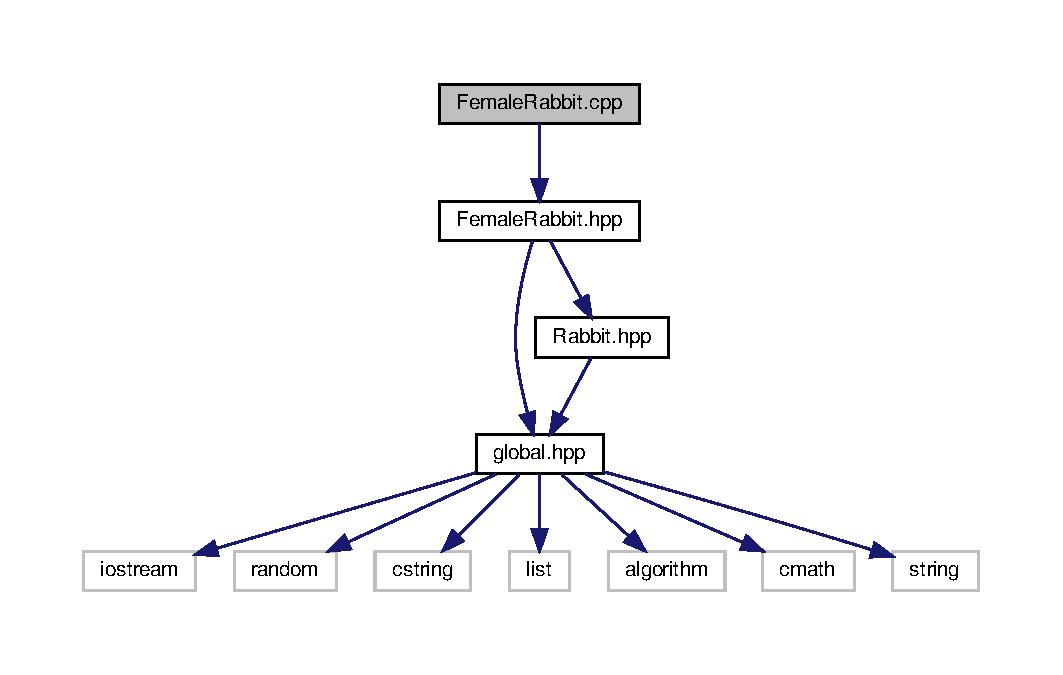
\includegraphics[width=350pt]{FemaleRabbit_8cpp__incl}
\end{center}
\end{figure}


\subsection{Description détaillée}
Fichier d\textquotesingle{}implémentation de la classe \hyperlink{classFemaleRabbit}{Female\+Rabbit}. 

\begin{DoxyAuthor}{Auteur}
Mathieu Arquilliere (\href{mailto:mathieu.arquilliere@etu.uca.fr}{\tt mathieu.\+arquilliere@etu.\+uca.\+fr}) 
\end{DoxyAuthor}
\begin{DoxyVersion}{Version}
0.\+1 
\end{DoxyVersion}
\begin{DoxyDate}{Date}
2019-\/11-\/17
\end{DoxyDate}
\begin{DoxyCopyright}{Copyright}
Copyright (c) 2019 
\end{DoxyCopyright}

\hypertarget{FemaleRabbit_8hpp}{}\section{Référence du fichier Female\+Rabbit.\+hpp}
\label{FemaleRabbit_8hpp}\index{Female\+Rabbit.\+hpp@{Female\+Rabbit.\+hpp}}


Fichier de déclaration de la classe \hyperlink{classFemaleRabbit}{Female\+Rabbit}.  


{\ttfamily \#include \char`\"{}global.\+hpp\char`\"{}}\newline
{\ttfamily \#include \char`\"{}Rabbit.\+hpp\char`\"{}}\newline
Graphe des dépendances par inclusion de Female\+Rabbit.\+hpp\+:
\nopagebreak
\begin{figure}[H]
\begin{center}
\leavevmode
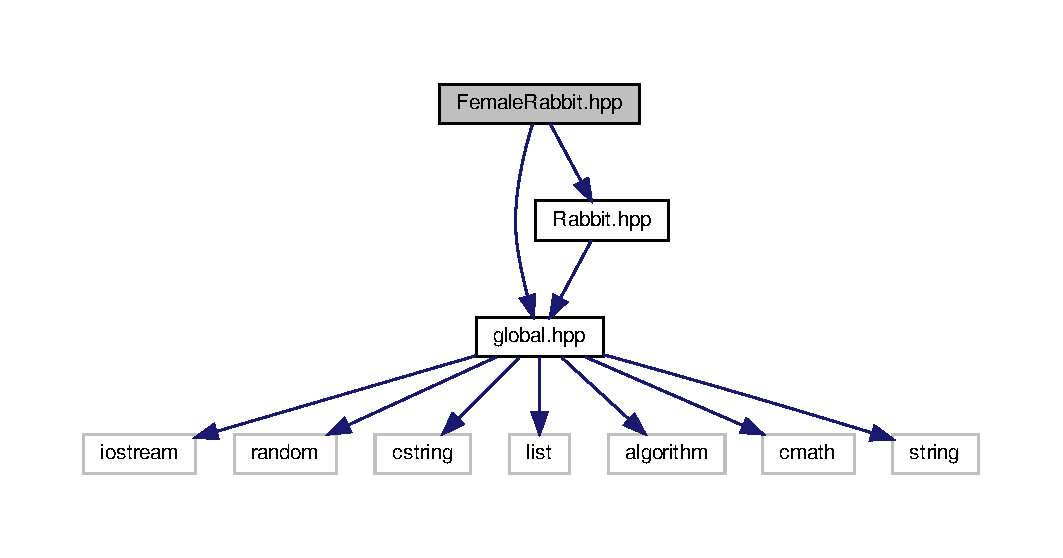
\includegraphics[width=350pt]{FemaleRabbit_8hpp__incl}
\end{center}
\end{figure}
Ce graphe montre quels fichiers incluent directement ou indirectement ce fichier \+:
\nopagebreak
\begin{figure}[H]
\begin{center}
\leavevmode
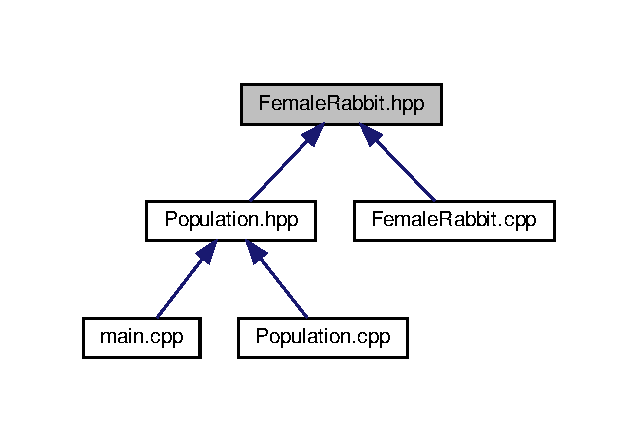
\includegraphics[width=306pt]{FemaleRabbit_8hpp__dep__incl}
\end{center}
\end{figure}
\subsection*{Structures de données}
\begin{DoxyCompactItemize}
\item 
class \hyperlink{classFemaleRabbit}{Female\+Rabbit}
\begin{DoxyCompactList}\small\item\em Classe représentant un lapin femelle. \end{DoxyCompactList}\end{DoxyCompactItemize}


\subsection{Description détaillée}
Fichier de déclaration de la classe \hyperlink{classFemaleRabbit}{Female\+Rabbit}. 

\begin{DoxyAuthor}{Auteur}
Mathieu Arquilliere (\href{mailto:mathieu.arquilliere@etu.uca.fr}{\tt mathieu.\+arquilliere@etu.\+uca.\+fr}) 
\end{DoxyAuthor}
\begin{DoxyVersion}{Version}
0.\+1 
\end{DoxyVersion}
\begin{DoxyDate}{Date}
2019-\/11-\/17
\end{DoxyDate}
\begin{DoxyCopyright}{Copyright}
Copyright (c) 2019 
\end{DoxyCopyright}

\hypertarget{global_8hpp}{}\section{Référence du fichier global.\+hpp}
\label{global_8hpp}\index{global.\+hpp@{global.\+hpp}}


Fichier d\textquotesingle{}include global pour que tous les fichiers ait accès aux includes et au distributions.  


{\ttfamily \#include $<$iostream$>$}\newline
{\ttfamily \#include $<$random$>$}\newline
{\ttfamily \#include $<$cstring$>$}\newline
{\ttfamily \#include $<$list$>$}\newline
{\ttfamily \#include $<$algorithm$>$}\newline
{\ttfamily \#include $<$cmath$>$}\newline
{\ttfamily \#include $<$string$>$}\newline
Graphe des dépendances par inclusion de global.\+hpp\+:
\nopagebreak
\begin{figure}[H]
\begin{center}
\leavevmode
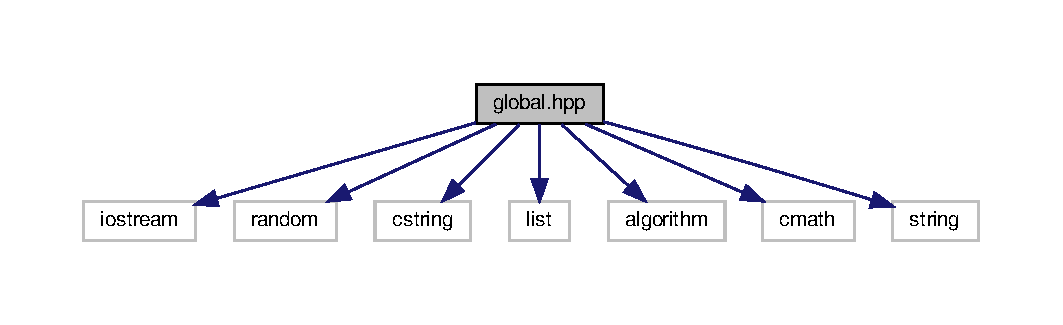
\includegraphics[width=350pt]{global_8hpp__incl}
\end{center}
\end{figure}
Ce graphe montre quels fichiers incluent directement ou indirectement ce fichier \+:
\nopagebreak
\begin{figure}[H]
\begin{center}
\leavevmode
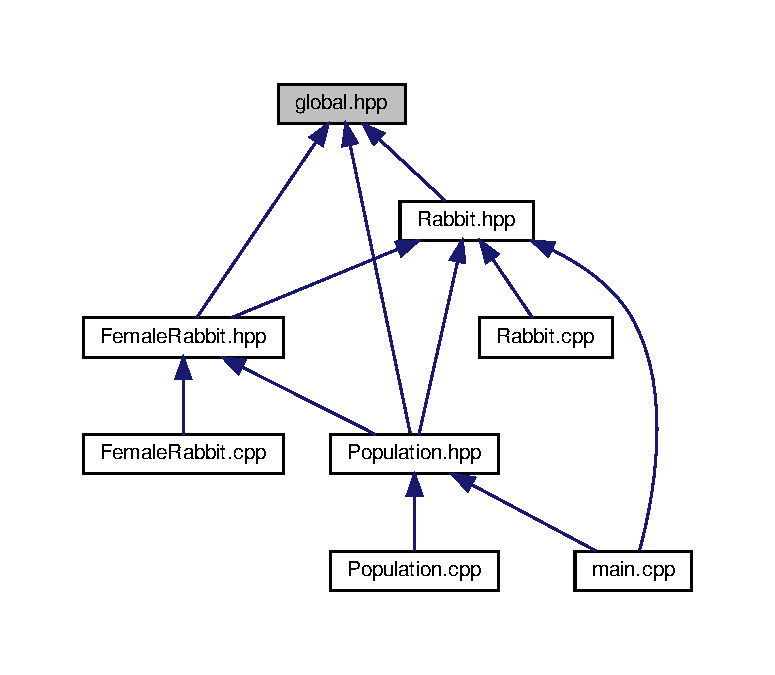
\includegraphics[width=350pt]{global_8hpp__dep__incl}
\end{center}
\end{figure}
\subsection*{Variables}
\begin{DoxyCompactItemize}
\item 
std\+::mt19937 \hyperlink{global_8hpp_a35141b83b1ff5df9c3aa9fb104eb906b}{generator}
\item 
std\+::uniform\+\_\+real\+\_\+distribution \hyperlink{global_8hpp_a30c25655b299c9f04fe054eb393d3690}{dis\+\_\+real\+\_\+0\+\_\+1}
\item 
std\+::uniform\+\_\+int\+\_\+distribution \hyperlink{global_8hpp_aa0c430aa1304ea1e210a3492724f484a}{dis\+\_\+int\+\_\+3\+\_\+6}
\item 
std\+::uniform\+\_\+int\+\_\+distribution \hyperlink{global_8hpp_a96625a3261ea5e001125b5240cfa7b4f}{dis\+\_\+int\+\_\+0\+\_\+11}
\item 
std\+::uniform\+\_\+int\+\_\+distribution \hyperlink{global_8hpp_a3f684258e2fe639454c3f3b51ad5761c}{dis\+\_\+int\+\_\+5\+\_\+8}
\item 
std\+::normal\+\_\+distribution \hyperlink{global_8hpp_a46324f02cd0355e7fce730e49b476d00}{dis\+\_\+normal\+\_\+6\+\_\+1}
\end{DoxyCompactItemize}


\subsection{Description détaillée}
Fichier d\textquotesingle{}include global pour que tous les fichiers ait accès aux includes et au distributions. 

\begin{DoxyAuthor}{Auteur}
Mathieu Arquilliere (\href{mailto:mathieu.arquilliere@etu.uca.fr}{\tt mathieu.\+arquilliere@etu.\+uca.\+fr}) 
\end{DoxyAuthor}
\begin{DoxyVersion}{Version}
0.\+1 
\end{DoxyVersion}
\begin{DoxyDate}{Date}
2019-\/11-\/18
\end{DoxyDate}
\begin{DoxyCopyright}{Copyright}
Copyright (c) 2019 
\end{DoxyCopyright}


\subsection{Documentation des variables}
\mbox{\Hypertarget{global_8hpp_a96625a3261ea5e001125b5240cfa7b4f}\label{global_8hpp_a96625a3261ea5e001125b5240cfa7b4f}} 
\index{global.\+hpp@{global.\+hpp}!dis\+\_\+int\+\_\+0\+\_\+11@{dis\+\_\+int\+\_\+0\+\_\+11}}
\index{dis\+\_\+int\+\_\+0\+\_\+11@{dis\+\_\+int\+\_\+0\+\_\+11}!global.\+hpp@{global.\+hpp}}
\subsubsection{\texorpdfstring{dis\+\_\+int\+\_\+0\+\_\+11}{dis\_int\_0\_11}}
{\footnotesize\ttfamily std\+::uniform\+\_\+int\+\_\+distribution dis\+\_\+int\+\_\+0\+\_\+11}

\mbox{\Hypertarget{global_8hpp_aa0c430aa1304ea1e210a3492724f484a}\label{global_8hpp_aa0c430aa1304ea1e210a3492724f484a}} 
\index{global.\+hpp@{global.\+hpp}!dis\+\_\+int\+\_\+3\+\_\+6@{dis\+\_\+int\+\_\+3\+\_\+6}}
\index{dis\+\_\+int\+\_\+3\+\_\+6@{dis\+\_\+int\+\_\+3\+\_\+6}!global.\+hpp@{global.\+hpp}}
\subsubsection{\texorpdfstring{dis\+\_\+int\+\_\+3\+\_\+6}{dis\_int\_3\_6}}
{\footnotesize\ttfamily std\+::uniform\+\_\+int\+\_\+distribution dis\+\_\+int\+\_\+3\+\_\+6}

\mbox{\Hypertarget{global_8hpp_a3f684258e2fe639454c3f3b51ad5761c}\label{global_8hpp_a3f684258e2fe639454c3f3b51ad5761c}} 
\index{global.\+hpp@{global.\+hpp}!dis\+\_\+int\+\_\+5\+\_\+8@{dis\+\_\+int\+\_\+5\+\_\+8}}
\index{dis\+\_\+int\+\_\+5\+\_\+8@{dis\+\_\+int\+\_\+5\+\_\+8}!global.\+hpp@{global.\+hpp}}
\subsubsection{\texorpdfstring{dis\+\_\+int\+\_\+5\+\_\+8}{dis\_int\_5\_8}}
{\footnotesize\ttfamily std\+::uniform\+\_\+int\+\_\+distribution dis\+\_\+int\+\_\+5\+\_\+8}

\mbox{\Hypertarget{global_8hpp_a46324f02cd0355e7fce730e49b476d00}\label{global_8hpp_a46324f02cd0355e7fce730e49b476d00}} 
\index{global.\+hpp@{global.\+hpp}!dis\+\_\+normal\+\_\+6\+\_\+1@{dis\+\_\+normal\+\_\+6\+\_\+1}}
\index{dis\+\_\+normal\+\_\+6\+\_\+1@{dis\+\_\+normal\+\_\+6\+\_\+1}!global.\+hpp@{global.\+hpp}}
\subsubsection{\texorpdfstring{dis\+\_\+normal\+\_\+6\+\_\+1}{dis\_normal\_6\_1}}
{\footnotesize\ttfamily std\+::normal\+\_\+distribution dis\+\_\+normal\+\_\+6\+\_\+1}

\mbox{\Hypertarget{global_8hpp_a30c25655b299c9f04fe054eb393d3690}\label{global_8hpp_a30c25655b299c9f04fe054eb393d3690}} 
\index{global.\+hpp@{global.\+hpp}!dis\+\_\+real\+\_\+0\+\_\+1@{dis\+\_\+real\+\_\+0\+\_\+1}}
\index{dis\+\_\+real\+\_\+0\+\_\+1@{dis\+\_\+real\+\_\+0\+\_\+1}!global.\+hpp@{global.\+hpp}}
\subsubsection{\texorpdfstring{dis\+\_\+real\+\_\+0\+\_\+1}{dis\_real\_0\_1}}
{\footnotesize\ttfamily std\+::uniform\+\_\+real\+\_\+distribution dis\+\_\+real\+\_\+0\+\_\+1}

\mbox{\Hypertarget{global_8hpp_a35141b83b1ff5df9c3aa9fb104eb906b}\label{global_8hpp_a35141b83b1ff5df9c3aa9fb104eb906b}} 
\index{global.\+hpp@{global.\+hpp}!generator@{generator}}
\index{generator@{generator}!global.\+hpp@{global.\+hpp}}
\subsubsection{\texorpdfstring{generator}{generator}}
{\footnotesize\ttfamily std\+::mt19937 generator}


\hypertarget{main_8cpp}{}\section{Référence du fichier main.\+cpp}
\label{main_8cpp}\index{main.\+cpp@{main.\+cpp}}


Fichier de tests pour les populations de lapins.  


{\ttfamily \#include $<$iostream$>$}\newline
{\ttfamily \#include $<$array$>$}\newline
{\ttfamily \#include \char`\"{}Rabbit.\+hpp\char`\"{}}\newline
{\ttfamily \#include \char`\"{}Population.\+hpp\char`\"{}}\newline
Graphe des dépendances par inclusion de main.\+cpp\+:
\nopagebreak
\begin{figure}[H]
\begin{center}
\leavevmode
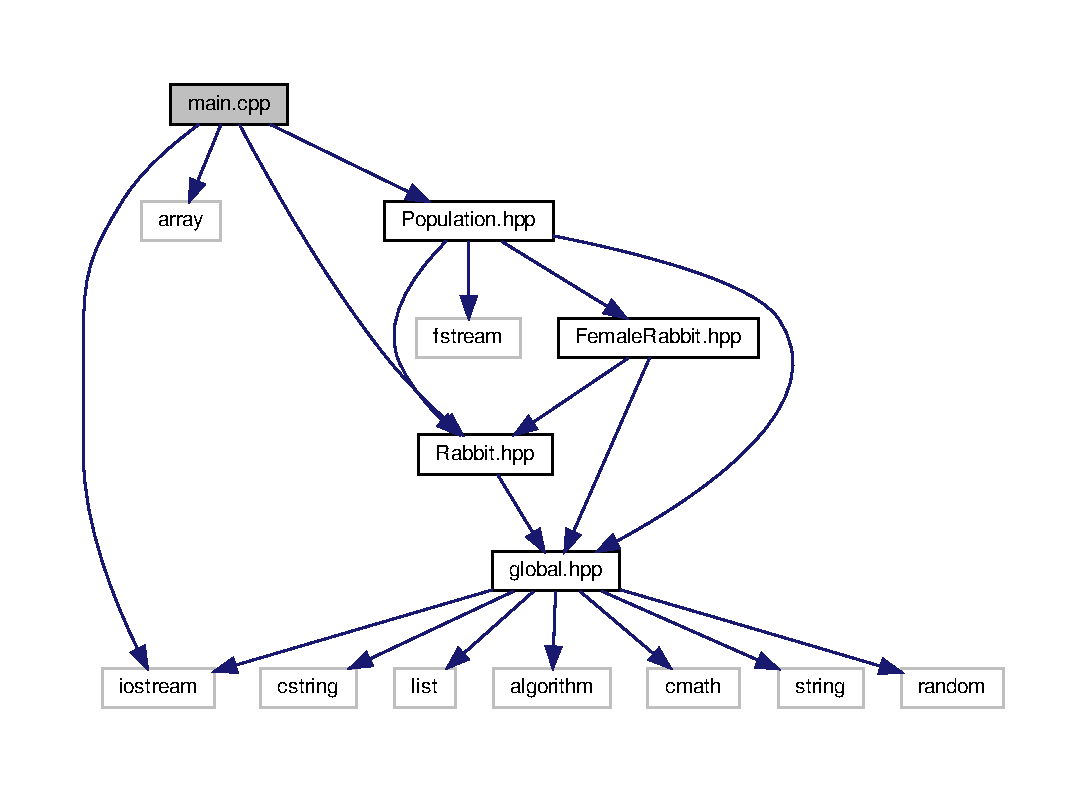
\includegraphics[width=350pt]{main_8cpp__incl}
\end{center}
\end{figure}
\subsection*{Fonctions}
\begin{DoxyCompactItemize}
\item 
std\+::mt19937 \hyperlink{main_8cpp_a71f02922c79d01461844507515cd1d75}{generator} (456)
\begin{DoxyCompactList}\small\item\em générateur de nombre aléatoire utilisant Mersenne Twister \end{DoxyCompactList}\item 
std\+::uniform\+\_\+real\+\_\+distribution \hyperlink{main_8cpp_a533b33accee6883724a3936388707491}{dis\+\_\+real\+\_\+0\+\_\+1} (0.\+0, 1.\+0)
\begin{DoxyCompactList}\small\item\em distribution réelle uniforme entre 0 et 1 \end{DoxyCompactList}\item 
std\+::uniform\+\_\+int\+\_\+distribution \hyperlink{main_8cpp_aea68d9df00e5881a3829f48f3c26ca6d}{dis\+\_\+int\+\_\+3\+\_\+6} (3, 6)
\begin{DoxyCompactList}\small\item\em distribution entière uniforme entre 3 et 6 (nombre de bébés dans chaque portée) \end{DoxyCompactList}\item 
std\+::uniform\+\_\+int\+\_\+distribution \hyperlink{main_8cpp_a3e9d5a0a4fc7b664c6b69d68ee03c920}{dis\+\_\+int\+\_\+0\+\_\+11} (0, 11)
\begin{DoxyCompactList}\small\item\em distribution entière uniforme entre 0 et 11 (mois auquel une femelle enfante) \end{DoxyCompactList}\item 
std\+::uniform\+\_\+int\+\_\+distribution \hyperlink{main_8cpp_a3a2201c154c797aaeb0221a29e655621}{dis\+\_\+int\+\_\+5\+\_\+8} (5, 8)
\begin{DoxyCompactList}\small\item\em distribution entière uniforme entre 5 et 8 (nombre de mois avant la majorité d\textquotesingle{}un lapin) \end{DoxyCompactList}\item 
std\+::normal\+\_\+distribution \hyperlink{main_8cpp_a6d17418f9f7681def106d4a92c10364b}{dis\+\_\+normal\+\_\+6\+\_\+1} (6, 1)
\begin{DoxyCompactList}\small\item\em distribution normale (nombre de portées d\textquotesingle{}une femelle dans l\textquotesingle{}année) \end{DoxyCompactList}\item 
int \hyperlink{main_8cpp_a0ddf1224851353fc92bfbff6f499fa97}{main} (int argc, char $\ast$argv\mbox{[}$\,$\mbox{]})
\end{DoxyCompactItemize}


\subsection{Description détaillée}
Fichier de tests pour les populations de lapins. 

\begin{DoxyAuthor}{Auteur}
Mathieu Arquilliere (\href{mailto:mathieu.arquilliere@etu.uca.fr}{\tt mathieu.\+arquilliere@etu.\+uca.\+fr}) 
\end{DoxyAuthor}
\begin{DoxyVersion}{Version}
0.\+1 
\end{DoxyVersion}
\begin{DoxyDate}{Date}
2019-\/11-\/17
\end{DoxyDate}
\begin{DoxyCopyright}{Copyright}
Copyright (c) 2019 
\end{DoxyCopyright}


\subsection{Documentation des fonctions}
\mbox{\Hypertarget{main_8cpp_a3e9d5a0a4fc7b664c6b69d68ee03c920}\label{main_8cpp_a3e9d5a0a4fc7b664c6b69d68ee03c920}} 
\index{main.\+cpp@{main.\+cpp}!dis\+\_\+int\+\_\+0\+\_\+11@{dis\+\_\+int\+\_\+0\+\_\+11}}
\index{dis\+\_\+int\+\_\+0\+\_\+11@{dis\+\_\+int\+\_\+0\+\_\+11}!main.\+cpp@{main.\+cpp}}
\subsubsection{\texorpdfstring{dis\+\_\+int\+\_\+0\+\_\+11()}{dis\_int\_0\_11()}}
{\footnotesize\ttfamily std\+::uniform\+\_\+int\+\_\+distribution dis\+\_\+int\+\_\+0\+\_\+11 (\begin{DoxyParamCaption}\item[{0}]{,  }\item[{11}]{ }\end{DoxyParamCaption})}



distribution entière uniforme entre 0 et 11 (mois auquel une femelle enfante) 

\mbox{\Hypertarget{main_8cpp_aea68d9df00e5881a3829f48f3c26ca6d}\label{main_8cpp_aea68d9df00e5881a3829f48f3c26ca6d}} 
\index{main.\+cpp@{main.\+cpp}!dis\+\_\+int\+\_\+3\+\_\+6@{dis\+\_\+int\+\_\+3\+\_\+6}}
\index{dis\+\_\+int\+\_\+3\+\_\+6@{dis\+\_\+int\+\_\+3\+\_\+6}!main.\+cpp@{main.\+cpp}}
\subsubsection{\texorpdfstring{dis\+\_\+int\+\_\+3\+\_\+6()}{dis\_int\_3\_6()}}
{\footnotesize\ttfamily std\+::uniform\+\_\+int\+\_\+distribution dis\+\_\+int\+\_\+3\+\_\+6 (\begin{DoxyParamCaption}\item[{3}]{,  }\item[{6}]{ }\end{DoxyParamCaption})}



distribution entière uniforme entre 3 et 6 (nombre de bébés dans chaque portée) 

\mbox{\Hypertarget{main_8cpp_a3a2201c154c797aaeb0221a29e655621}\label{main_8cpp_a3a2201c154c797aaeb0221a29e655621}} 
\index{main.\+cpp@{main.\+cpp}!dis\+\_\+int\+\_\+5\+\_\+8@{dis\+\_\+int\+\_\+5\+\_\+8}}
\index{dis\+\_\+int\+\_\+5\+\_\+8@{dis\+\_\+int\+\_\+5\+\_\+8}!main.\+cpp@{main.\+cpp}}
\subsubsection{\texorpdfstring{dis\+\_\+int\+\_\+5\+\_\+8()}{dis\_int\_5\_8()}}
{\footnotesize\ttfamily std\+::uniform\+\_\+int\+\_\+distribution dis\+\_\+int\+\_\+5\+\_\+8 (\begin{DoxyParamCaption}\item[{5}]{,  }\item[{8}]{ }\end{DoxyParamCaption})}



distribution entière uniforme entre 5 et 8 (nombre de mois avant la majorité d\textquotesingle{}un lapin) 

\mbox{\Hypertarget{main_8cpp_a6d17418f9f7681def106d4a92c10364b}\label{main_8cpp_a6d17418f9f7681def106d4a92c10364b}} 
\index{main.\+cpp@{main.\+cpp}!dis\+\_\+normal\+\_\+6\+\_\+1@{dis\+\_\+normal\+\_\+6\+\_\+1}}
\index{dis\+\_\+normal\+\_\+6\+\_\+1@{dis\+\_\+normal\+\_\+6\+\_\+1}!main.\+cpp@{main.\+cpp}}
\subsubsection{\texorpdfstring{dis\+\_\+normal\+\_\+6\+\_\+1()}{dis\_normal\_6\_1()}}
{\footnotesize\ttfamily std\+::normal\+\_\+distribution dis\+\_\+normal\+\_\+6\+\_\+1 (\begin{DoxyParamCaption}\item[{6}]{,  }\item[{1}]{ }\end{DoxyParamCaption})}



distribution normale (nombre de portées d\textquotesingle{}une femelle dans l\textquotesingle{}année) 

\mbox{\Hypertarget{main_8cpp_a533b33accee6883724a3936388707491}\label{main_8cpp_a533b33accee6883724a3936388707491}} 
\index{main.\+cpp@{main.\+cpp}!dis\+\_\+real\+\_\+0\+\_\+1@{dis\+\_\+real\+\_\+0\+\_\+1}}
\index{dis\+\_\+real\+\_\+0\+\_\+1@{dis\+\_\+real\+\_\+0\+\_\+1}!main.\+cpp@{main.\+cpp}}
\subsubsection{\texorpdfstring{dis\+\_\+real\+\_\+0\+\_\+1()}{dis\_real\_0\_1()}}
{\footnotesize\ttfamily std\+::uniform\+\_\+real\+\_\+distribution dis\+\_\+real\+\_\+0\+\_\+1 (\begin{DoxyParamCaption}\item[{0.}]{0,  }\item[{1.}]{0 }\end{DoxyParamCaption})}



distribution réelle uniforme entre 0 et 1 

\mbox{\Hypertarget{main_8cpp_a71f02922c79d01461844507515cd1d75}\label{main_8cpp_a71f02922c79d01461844507515cd1d75}} 
\index{main.\+cpp@{main.\+cpp}!generator@{generator}}
\index{generator@{generator}!main.\+cpp@{main.\+cpp}}
\subsubsection{\texorpdfstring{generator()}{generator()}}
{\footnotesize\ttfamily std\+::mt19937 generator (\begin{DoxyParamCaption}\item[{456}]{ }\end{DoxyParamCaption})}



générateur de nombre aléatoire utilisant Mersenne Twister 

\mbox{\Hypertarget{main_8cpp_a0ddf1224851353fc92bfbff6f499fa97}\label{main_8cpp_a0ddf1224851353fc92bfbff6f499fa97}} 
\index{main.\+cpp@{main.\+cpp}!main@{main}}
\index{main@{main}!main.\+cpp@{main.\+cpp}}
\subsubsection{\texorpdfstring{main()}{main()}}
{\footnotesize\ttfamily int main (\begin{DoxyParamCaption}\item[{int}]{argc,  }\item[{char $\ast$}]{argv\mbox{[}$\,$\mbox{]} }\end{DoxyParamCaption})}



Définition à la ligne 46 du fichier main.\+cpp.

Voici le graphe d\textquotesingle{}appel pour cette fonction \+:
\nopagebreak
\begin{figure}[H]
\begin{center}
\leavevmode
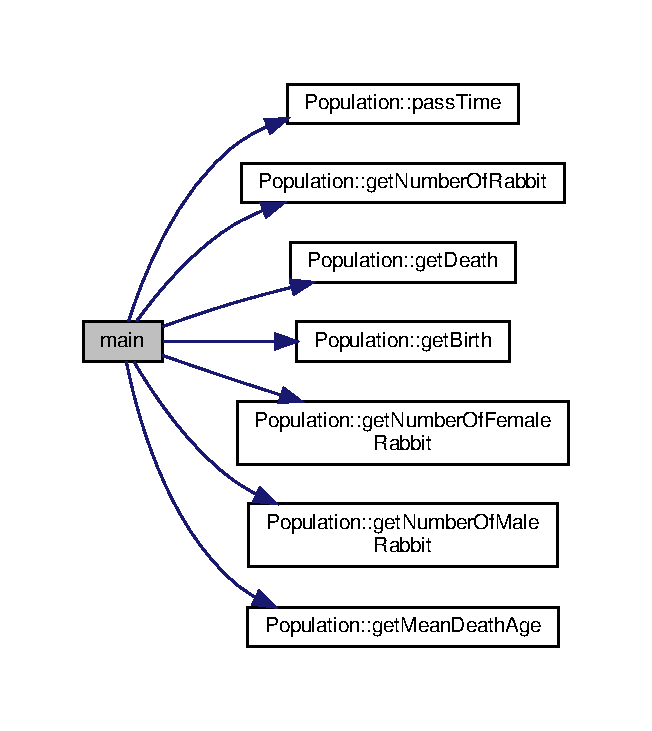
\includegraphics[width=313pt]{main_8cpp_a0ddf1224851353fc92bfbff6f499fa97_cgraph}
\end{center}
\end{figure}

\hypertarget{Population_8cpp}{}\section{Référence du fichier Population.\+cpp}
\label{Population_8cpp}\index{Population.\+cpp@{Population.\+cpp}}


Fichier d\textquotesingle{}implémentation de la classe \hyperlink{classPopulation}{Population}.  


{\ttfamily \#include \char`\"{}Population.\+hpp\char`\"{}}\newline
Graphe des dépendances par inclusion de Population.\+cpp\+:
\nopagebreak
\begin{figure}[H]
\begin{center}
\leavevmode
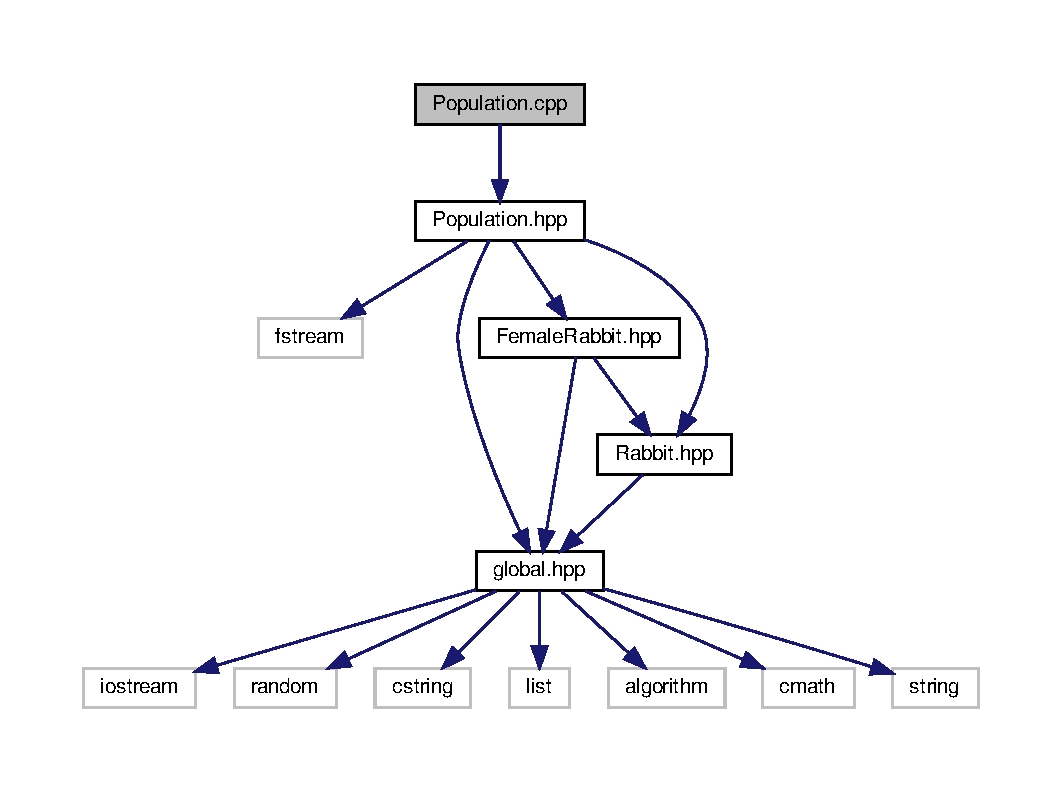
\includegraphics[width=350pt]{Population_8cpp__incl}
\end{center}
\end{figure}
\subsection*{Fonctions}
\begin{DoxyCompactItemize}
\item 
std\+::ostream \& \hyperlink{Population_8cpp_acbf3a497ada86e986186c14dd53ac905}{operator$<$$<$} (std\+::ostream \&out, \hyperlink{classPopulation}{Population} const \&pop)
\begin{DoxyCompactList}\small\item\em surcharge de l\textquotesingle{}opérateur $<$$<$ \end{DoxyCompactList}\end{DoxyCompactItemize}


\subsection{Description détaillée}
Fichier d\textquotesingle{}implémentation de la classe \hyperlink{classPopulation}{Population}. 

\begin{DoxyAuthor}{Auteur}
Mathieu Arquilliere (\href{mailto:mathieu.arquilliere@etu.uca.fr}{\tt mathieu.\+arquilliere@etu.\+uca.\+fr}) 
\end{DoxyAuthor}
\begin{DoxyVersion}{Version}
0.\+1 
\end{DoxyVersion}
\begin{DoxyDate}{Date}
2019-\/11-\/17
\end{DoxyDate}
\begin{DoxyCopyright}{Copyright}
Copyright (c) 2019 
\end{DoxyCopyright}


\subsection{Documentation des fonctions}
\mbox{\Hypertarget{Population_8cpp_acbf3a497ada86e986186c14dd53ac905}\label{Population_8cpp_acbf3a497ada86e986186c14dd53ac905}} 
\index{Population.\+cpp@{Population.\+cpp}!operator$<$$<$@{operator$<$$<$}}
\index{operator$<$$<$@{operator$<$$<$}!Population.\+cpp@{Population.\+cpp}}
\subsubsection{\texorpdfstring{operator$<$$<$()}{operator<<()}}
{\footnotesize\ttfamily std\+::ostream\& operator$<$$<$ (\begin{DoxyParamCaption}\item[{std\+::ostream \&}]{out,  }\item[{\hyperlink{classPopulation}{Population} const \&}]{pop }\end{DoxyParamCaption})}



surcharge de l\textquotesingle{}opérateur $<$$<$ 

Ecrit dans un flux donné l\textquotesingle{}état actuel de la population


\begin{DoxyParams}[1]{Paramètres}
\mbox{\tt in}  & {\em out} & flux de sortie dans lequel on écrit \\
\hline
\mbox{\tt in}  & {\em pop} & population dont on veut écrire l\textquotesingle{}état \\
\hline
\end{DoxyParams}
\begin{DoxyReturn}{Renvoie}
std\+::ostream\& flux de sortie 
\end{DoxyReturn}


Définition à la ligne 206 du fichier Population.\+cpp.

Voici le graphe d\textquotesingle{}appel pour cette fonction \+:
\nopagebreak
\begin{figure}[H]
\begin{center}
\leavevmode
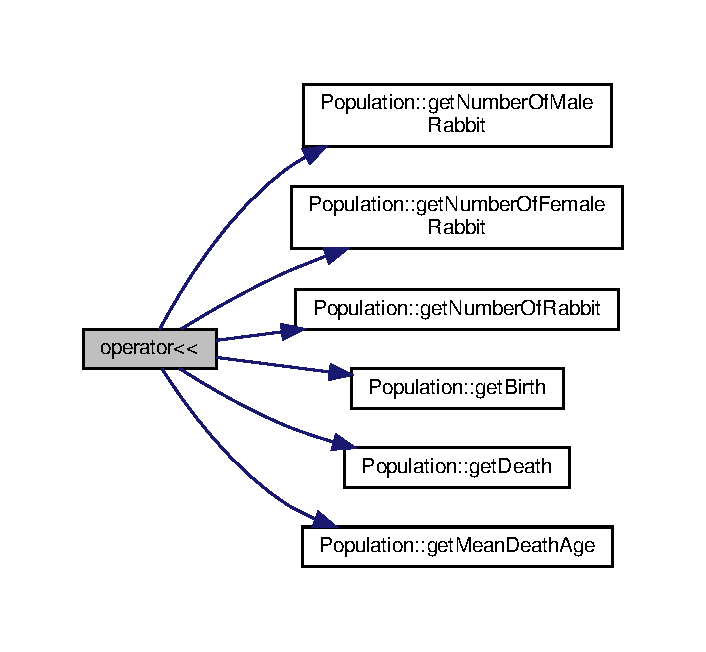
\includegraphics[width=339pt]{Population_8cpp_acbf3a497ada86e986186c14dd53ac905_cgraph}
\end{center}
\end{figure}

\hypertarget{Population_8hpp}{}\section{Référence du fichier Population.\+hpp}
\label{Population_8hpp}\index{Population.\+hpp@{Population.\+hpp}}


Fichier de déclaration de la classe \hyperlink{classPopulation}{Population}.  


{\ttfamily \#include $<$fstream$>$}\newline
{\ttfamily \#include \char`\"{}global.\+hpp\char`\"{}}\newline
{\ttfamily \#include \char`\"{}Female\+Rabbit.\+hpp\char`\"{}}\newline
{\ttfamily \#include \char`\"{}Rabbit.\+hpp\char`\"{}}\newline
Graphe des dépendances par inclusion de Population.\+hpp\+:
\nopagebreak
\begin{figure}[H]
\begin{center}
\leavevmode
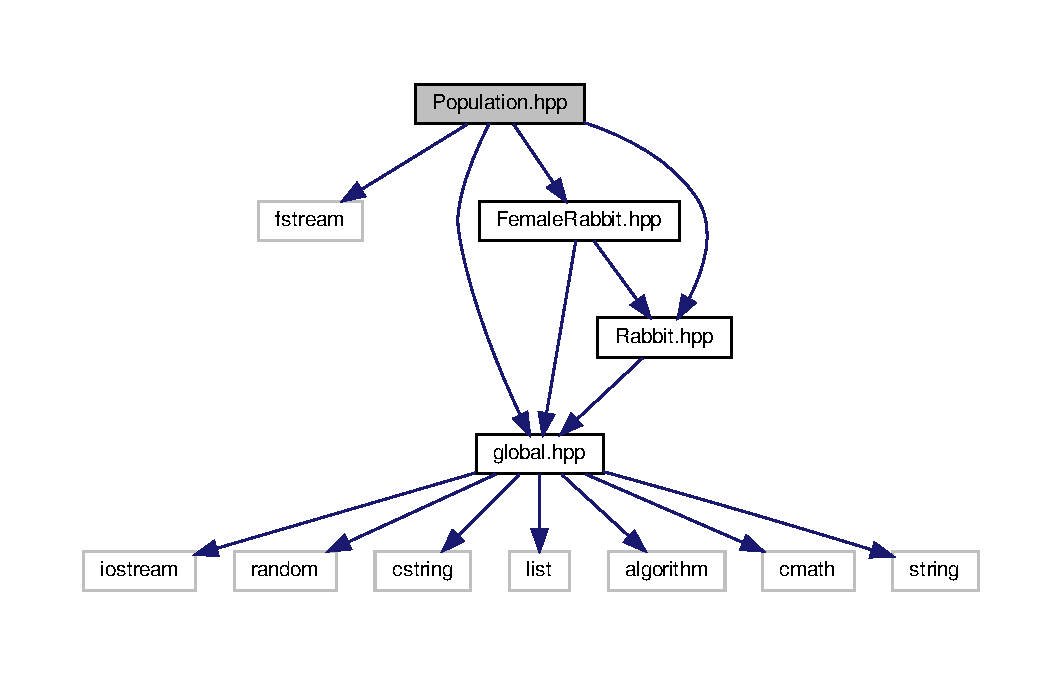
\includegraphics[width=350pt]{Population_8hpp__incl}
\end{center}
\end{figure}
Ce graphe montre quels fichiers incluent directement ou indirectement ce fichier \+:
\nopagebreak
\begin{figure}[H]
\begin{center}
\leavevmode
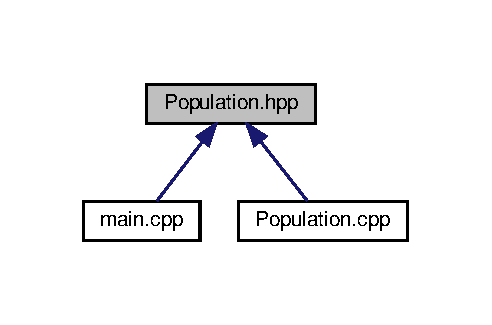
\includegraphics[width=236pt]{Population_8hpp__dep__incl}
\end{center}
\end{figure}
\subsection*{Structures de données}
\begin{DoxyCompactItemize}
\item 
class \hyperlink{classPopulation}{Population}
\begin{DoxyCompactList}\small\item\em Représente une population de lapins. \end{DoxyCompactList}\end{DoxyCompactItemize}
\subsection*{Fonctions}
\begin{DoxyCompactItemize}
\item 
std\+::ostream \& \hyperlink{Population_8hpp_acbf3a497ada86e986186c14dd53ac905}{operator$<$$<$} (std\+::ostream \&out, \hyperlink{classPopulation}{Population} const \&pop)
\begin{DoxyCompactList}\small\item\em surcharge de l\textquotesingle{}opérateur $<$$<$ \end{DoxyCompactList}\end{DoxyCompactItemize}


\subsection{Description détaillée}
Fichier de déclaration de la classe \hyperlink{classPopulation}{Population}. 

\begin{DoxyAuthor}{Auteur}
Mathieu Arquilliere (\href{mailto:mathieu.arquilliere@etu.uca.fr}{\tt mathieu.\+arquilliere@etu.\+uca.\+fr}) 
\end{DoxyAuthor}
\begin{DoxyVersion}{Version}
0.\+1 
\end{DoxyVersion}
\begin{DoxyDate}{Date}
2019-\/11-\/17
\end{DoxyDate}
\begin{DoxyCopyright}{Copyright}
Copyright (c) 2019 
\end{DoxyCopyright}


\subsection{Documentation des fonctions}
\mbox{\Hypertarget{Population_8hpp_acbf3a497ada86e986186c14dd53ac905}\label{Population_8hpp_acbf3a497ada86e986186c14dd53ac905}} 
\index{Population.\+hpp@{Population.\+hpp}!operator$<$$<$@{operator$<$$<$}}
\index{operator$<$$<$@{operator$<$$<$}!Population.\+hpp@{Population.\+hpp}}
\subsubsection{\texorpdfstring{operator$<$$<$()}{operator<<()}}
{\footnotesize\ttfamily std\+::ostream\& operator$<$$<$ (\begin{DoxyParamCaption}\item[{std\+::ostream \&}]{out,  }\item[{\hyperlink{classPopulation}{Population} const \&}]{pop }\end{DoxyParamCaption})}



surcharge de l\textquotesingle{}opérateur $<$$<$ 

Ecrit dans un flux donné l\textquotesingle{}état actuel de la population


\begin{DoxyParams}[1]{Paramètres}
\mbox{\tt in}  & {\em out} & flux de sortie dans lequel on écrit \\
\hline
\mbox{\tt in}  & {\em pop} & population dont on veut écrire l\textquotesingle{}état \\
\hline
\end{DoxyParams}
\begin{DoxyReturn}{Renvoie}
std\+::ostream\& flux de sortie 
\end{DoxyReturn}


Définition à la ligne 206 du fichier Population.\+cpp.

Voici le graphe d\textquotesingle{}appel pour cette fonction \+:
\nopagebreak
\begin{figure}[H]
\begin{center}
\leavevmode
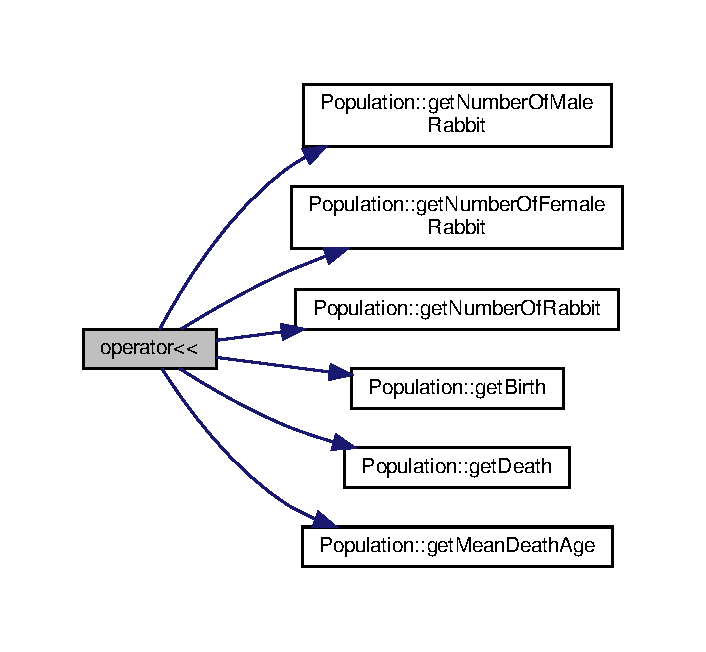
\includegraphics[width=339pt]{Population_8hpp_acbf3a497ada86e986186c14dd53ac905_cgraph}
\end{center}
\end{figure}

\hypertarget{Rabbit_8cpp}{}\section{Référence du fichier Rabbit.\+cpp}
\label{Rabbit_8cpp}\index{Rabbit.\+cpp@{Rabbit.\+cpp}}


Fichier d\textquotesingle{}implémentation de la classe \hyperlink{classRabbit}{Rabbit}.  


{\ttfamily \#include \char`\"{}Rabbit.\+hpp\char`\"{}}\newline
Graphe des dépendances par inclusion de Rabbit.\+cpp\+:
\nopagebreak
\begin{figure}[H]
\begin{center}
\leavevmode
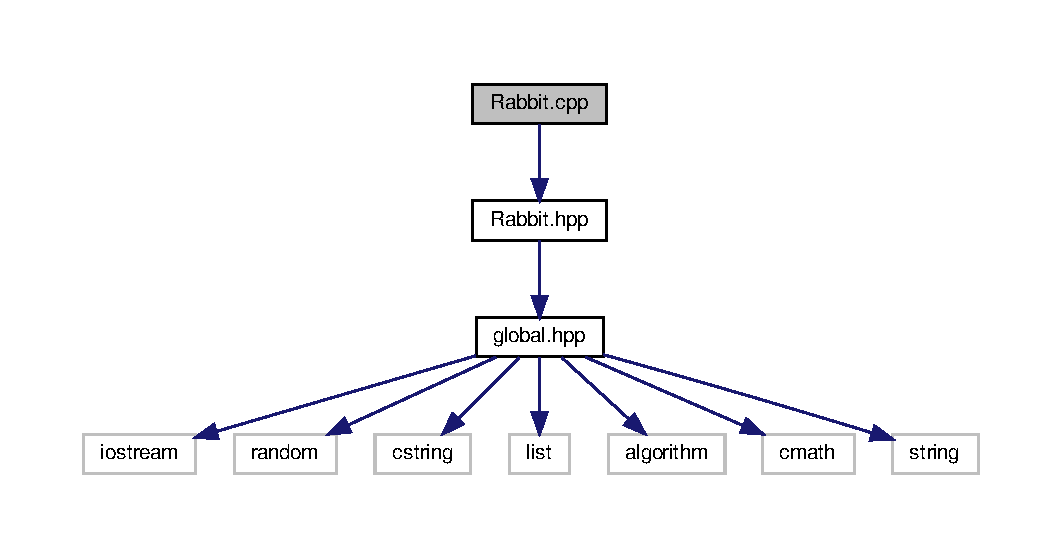
\includegraphics[width=350pt]{Rabbit_8cpp__incl}
\end{center}
\end{figure}


\subsection{Description détaillée}
Fichier d\textquotesingle{}implémentation de la classe \hyperlink{classRabbit}{Rabbit}. 

\begin{DoxyAuthor}{Auteur}
Mathieu Arquilliere (\href{mailto:mathieu.arquilliere@etu.uca.fr}{\tt mathieu.\+arquilliere@etu.\+uca.\+fr}) 
\end{DoxyAuthor}
\begin{DoxyVersion}{Version}
0.\+1 
\end{DoxyVersion}
\begin{DoxyDate}{Date}
2019-\/11-\/17
\end{DoxyDate}
\begin{DoxyCopyright}{Copyright}
Copyright (c) 2019 
\end{DoxyCopyright}

\hypertarget{Rabbit_8hpp}{}\section{Référence du fichier Rabbit.\+hpp}
\label{Rabbit_8hpp}\index{Rabbit.\+hpp@{Rabbit.\+hpp}}


Classe déclarant le comportement d\textquotesingle{}un beau et fort lapin. Contient également l\textquotesingle{}ensembles des distributions nécessaires à la simulation.  


{\ttfamily \#include $<$iostream$>$}\newline
{\ttfamily \#include $<$string$>$}\newline
{\ttfamily \#include $<$vector$>$}\newline
{\ttfamily \#include $<$random$>$}\newline
{\ttfamily \#include $<$array$>$}\newline
Graphe des dépendances par inclusion de Rabbit.\+hpp\+:\nopagebreak
\begin{figure}[H]
\begin{center}
\leavevmode
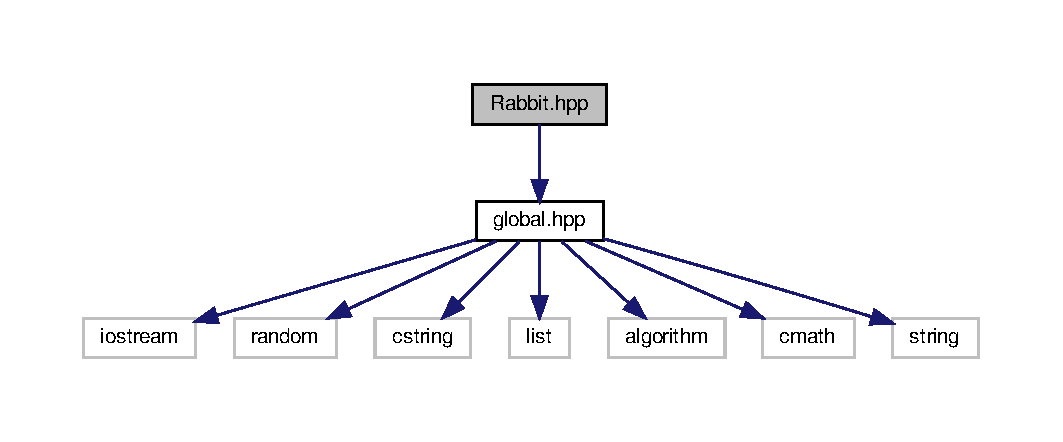
\includegraphics[width=350pt]{Rabbit_8hpp__incl}
\end{center}
\end{figure}
Ce graphe montre quels fichiers incluent directement ou indirectement ce fichier \+:
\nopagebreak
\begin{figure}[H]
\begin{center}
\leavevmode
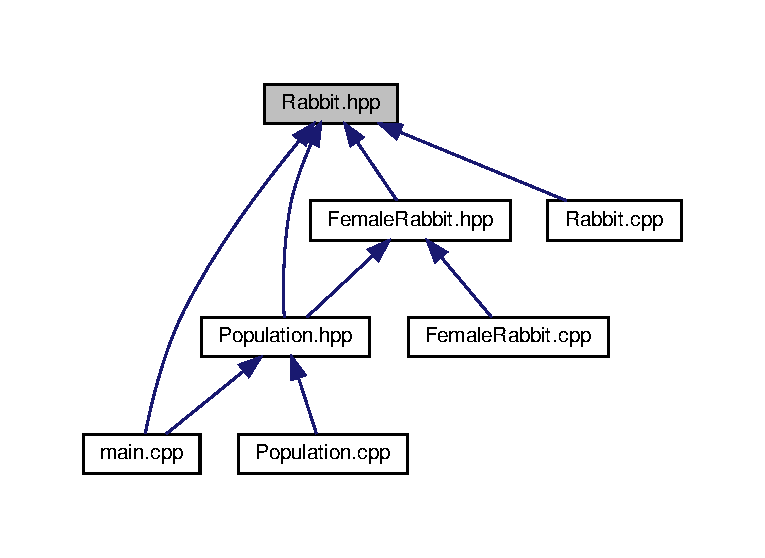
\includegraphics[width=341pt]{Rabbit_8hpp__dep__incl}
\end{center}
\end{figure}
\subsection*{Classes}
\begin{DoxyCompactItemize}
\item 
class \hyperlink{classRabbit}{Rabbit}
\end{DoxyCompactItemize}


\subsection{Description détaillée}
Classe déclarant le comportement d\textquotesingle{}un beau et fort lapin. Contient également l\textquotesingle{}ensembles des distributions nécessaires à la simulation. 

\begin{DoxyAuthor}{Auteur}
Jérémy Z\+A\+N\+G\+LA (\href{mailto:zangla.jeremy@gmail.com}{\tt zangla.\+jeremy@gmail.\+com}) 
\end{DoxyAuthor}
\begin{DoxyVersion}{Version}
1 
\end{DoxyVersion}
\begin{DoxyDate}{Date}
2019-\/11-\/16
\end{DoxyDate}
\begin{DoxyCopyright}{Copyright}
Copyright (c) 2019 
\end{DoxyCopyright}

%--- End generated contents ---

% Index
\backmatter
\newpage
\phantomsection
\clearemptydoublepage
\addcontentsline{toc}{chapter}{Index}
\printindex

\end{document}
